% Preamble and title-block layout reused from the author's previous Apart sprint report (pre-existing).
\documentclass[11pt,letterpaper]{article}
\usepackage[margin=1in]{geometry}
\usepackage{fontspec}
\setmainfont{GFSDidot}[Extension=.otf, UprightFont=*, BoldFont=*Bold, ItalicFont=*Italic, BoldItalicFont=*BoldItalic]
\setmonofont{lmmono10-regular.otf}[Scale=0.95]
\usepackage{microtype}
\usepackage{amsmath}
\usepackage{graphicx}
\usepackage{booktabs}
\usepackage{array}
\usepackage{tabularx}
\usepackage[labelsep=colon,font=small]{caption}
\usepackage{enumitem}
\usepackage{titlesec}
\usepackage{xcolor}
\usepackage{float}
\usepackage[hidelinks]{hyperref}
\sloppy
\usepackage{xurl}
\setlength{\parindent}{0pt}
\setlength{\parskip}{4pt}
\titleformat{\section}{\Large}{\thesection.}{0.45em}{}
\titlespacing*{\section}{0pt}{11pt}{3pt}
\titleformat{\subsection}{\large}{\thesubsection}{0.45em}{}
\titlespacing*{\subsection}{0pt}{7pt}{2pt}
\setlist{nosep,leftmargin=1.4em,topsep=2pt}
\newcommand{\head}[1]{\textbf{#1}\hspace{0.3em}}
\graphicspath{{../../results/main/figures/}}
\renewcommand{\thefootnote}{\arabic{footnote}}
% generated by src/analysis/tex_numbers.py from results/main/report_numbers.json; do not edit
\newcommand{\nFRFleetMzero}{0.0}
\newcommand{\nFRloFleetMzero}{0.0}
\newcommand{\nFRhiFleetMzero}{0.0}
\newcommand{\nFRFleetMone}{0.0}
\newcommand{\nFRloFleetMone}{0.0}
\newcommand{\nFRhiFleetMone}{0.0}
\newcommand{\nFRFleetMtwo}{68.1}
\newcommand{\nFRloFleetMtwo}{64.7}
\newcommand{\nFRhiFleetMtwo}{71.3}
\newcommand{\nFRFleetMtwob}{56.2}
\newcommand{\nFRloFleetMtwob}{51.3}
\newcommand{\nFRhiFleetMtwob}{61.0}
\newcommand{\nFRFleetMthree}{5.1}
\newcommand{\nFRloFleetMthree}{3.9}
\newcommand{\nFRhiFleetMthree}{6.5}
\newcommand{\nFRFleetMthreew}{3.3}
\newcommand{\nFRloFleetMthreew}{2.6}
\newcommand{\nFRhiFleetMthreew}{4.0}
\newcommand{\nFRFleetMfour}{2.6}
\newcommand{\nFRloFleetMfour}{1.7}
\newcommand{\nFRhiFleetMfour}{3.5}
\newcommand{\nFRFleetMfourj}{2.1}
\newcommand{\nFRloFleetMfourj}{1.6}
\newcommand{\nFRhiFleetMfourj}{2.7}
\newcommand{\nFRFleetMfourr}{3.0}
\newcommand{\nFRloFleetMfourr}{2.1}
\newcommand{\nFRhiFleetMfourr}{4.0}
\newcommand{\nFRFleetdriftMzero}{0.0}
\newcommand{\nFRloFleetdriftMzero}{0.0}
\newcommand{\nFRhiFleetdriftMzero}{0.0}
\newcommand{\nFRFleetdriftMone}{0.0}
\newcommand{\nFRloFleetdriftMone}{0.0}
\newcommand{\nFRhiFleetdriftMone}{0.0}
\newcommand{\nFRFleetdriftMtwo}{70.7}
\newcommand{\nFRloFleetdriftMtwo}{66.4}
\newcommand{\nFRhiFleetdriftMtwo}{75.3}
\newcommand{\nFRFleetdriftMtwob}{59.7}
\newcommand{\nFRloFleetdriftMtwob}{53.0}
\newcommand{\nFRhiFleetdriftMtwob}{66.1}
\newcommand{\nFRFleetdriftMthree}{5.9}
\newcommand{\nFRloFleetdriftMthree}{3.5}
\newcommand{\nFRhiFleetdriftMthree}{8.5}
\newcommand{\nFRFleetdriftMthreew}{3.1}
\newcommand{\nFRloFleetdriftMthreew}{1.9}
\newcommand{\nFRhiFleetdriftMthreew}{4.5}
\newcommand{\nFRFleetdriftMfour}{64.3}
\newcommand{\nFRloFleetdriftMfour}{54.4}
\newcommand{\nFRhiFleetdriftMfour}{73.0}
\newcommand{\nFRFleetdriftMfourj}{1.8}
\newcommand{\nFRloFleetdriftMfourj}{1.2}
\newcommand{\nFRhiFleetdriftMfourj}{2.4}
\newcommand{\nFRFleetdriftMfourr}{36.7}
\newcommand{\nFRloFleetdriftMfourr}{30.9}
\newcommand{\nFRhiFleetdriftMfourr}{42.4}
\newcommand{\nFRIndependentMzero}{0.0}
\newcommand{\nFRloIndependentMzero}{0.0}
\newcommand{\nFRhiIndependentMzero}{0.0}
\newcommand{\nFRIndependentMone}{0.0}
\newcommand{\nFRloIndependentMone}{0.0}
\newcommand{\nFRhiIndependentMone}{0.0}
\newcommand{\nFRIndependentMtwo}{7.2}
\newcommand{\nFRloIndependentMtwo}{5.7}
\newcommand{\nFRhiIndependentMtwo}{8.7}
\newcommand{\nFRIndependentMtwob}{7.2}
\newcommand{\nFRloIndependentMtwob}{5.2}
\newcommand{\nFRhiIndependentMtwob}{9.4}
\newcommand{\nFRIndependentMthree}{5.5}
\newcommand{\nFRloIndependentMthree}{4.2}
\newcommand{\nFRhiIndependentMthree}{6.9}
\newcommand{\nFRIndependentMthreew}{29.8}
\newcommand{\nFRloIndependentMthreew}{26.8}
\newcommand{\nFRhiIndependentMthreew}{33.3}
\newcommand{\nFRIndependentMfour}{0.2}
\newcommand{\nFRloIndependentMfour}{0.0}
\newcommand{\nFRhiIndependentMfour}{0.5}
\newcommand{\nFRIndependentMfourr}{1.6}
\newcommand{\nFRloIndependentMfourr}{1.0}
\newcommand{\nFRhiIndependentMfourr}{2.2}
\newcommand{\nFRSwarmMzero}{97.0}
\newcommand{\nFRloSwarmMzero}{95.0}
\newcommand{\nFRhiSwarmMzero}{98.7}
\newcommand{\nFRSwarmMone}{0.0}
\newcommand{\nFRloSwarmMone}{0.0}
\newcommand{\nFRhiSwarmMone}{0.0}
\newcommand{\nFRSwarmMtwo}{35.9}
\newcommand{\nFRloSwarmMtwo}{33.0}
\newcommand{\nFRhiSwarmMtwo}{38.9}
\newcommand{\nFRSwarmMtwob}{0.8}
\newcommand{\nFRloSwarmMtwob}{0.5}
\newcommand{\nFRhiSwarmMtwob}{1.1}
\newcommand{\nFRSwarmMthree}{1.6}
\newcommand{\nFRloSwarmMthree}{1.1}
\newcommand{\nFRhiSwarmMthree}{2.1}
\newcommand{\nFRSwarmMthreew}{10.3}
\newcommand{\nFRloSwarmMthreew}{9.1}
\newcommand{\nFRhiSwarmMthreew}{11.6}
\newcommand{\nFRSwarmMfour}{11.7}
\newcommand{\nFRloSwarmMfour}{9.7}
\newcommand{\nFRhiSwarmMfour}{14.1}
\newcommand{\nFRSwarmMfourj}{3.6}
\newcommand{\nFRloSwarmMfourj}{2.9}
\newcommand{\nFRhiSwarmMfourj}{4.4}
\newcommand{\nFRSwarmMfourr}{3.3}
\newcommand{\nFRloSwarmMfourr}{2.5}
\newcommand{\nFRhiSwarmMfourr}{4.1}
\newcommand{\nFRTacitMzero}{0.0}
\newcommand{\nFRloTacitMzero}{0.0}
\newcommand{\nFRhiTacitMzero}{0.0}
\newcommand{\nFRTacitMone}{0.0}
\newcommand{\nFRloTacitMone}{0.0}
\newcommand{\nFRhiTacitMone}{0.0}
\newcommand{\nFRTacitMtwo}{16.0}
\newcommand{\nFRloTacitMtwo}{14.2}
\newcommand{\nFRhiTacitMtwo}{17.9}
\newcommand{\nFRTacitMtwob}{13.3}
\newcommand{\nFRloTacitMtwob}{11.0}
\newcommand{\nFRhiTacitMtwob}{15.7}
\newcommand{\nFRTacitMthree}{2.2}
\newcommand{\nFRloTacitMthree}{1.3}
\newcommand{\nFRhiTacitMthree}{3.3}
\newcommand{\nFRTacitMthreew}{16.1}
\newcommand{\nFRloTacitMthreew}{11.1}
\newcommand{\nFRhiTacitMthreew}{21.2}
\newcommand{\nFRTacitMfour}{3.5}
\newcommand{\nFRloTacitMfour}{2.5}
\newcommand{\nFRhiTacitMfour}{4.6}
\newcommand{\nFRTacitMfourj}{2.8}
\newcommand{\nFRloTacitMfourj}{1.7}
\newcommand{\nFRhiTacitMfourj}{4.0}
\newcommand{\nFRTacitMfourr}{3.3}
\newcommand{\nFRloTacitMfourr}{2.2}
\newcommand{\nFRhiTacitMfourr}{4.3}
\newcommand{\nFRUninstructedMzero}{62.2}
\newcommand{\nFRloUninstructedMzero}{62.2}
\newcommand{\nFRhiUninstructedMzero}{62.2}
\newcommand{\nFRUninstructedMone}{0.0}
\newcommand{\nFRloUninstructedMone}{0.0}
\newcommand{\nFRhiUninstructedMone}{0.0}
\newcommand{\nFRUninstructedMtwo}{43.9}
\newcommand{\nFRloUninstructedMtwo}{40.1}
\newcommand{\nFRhiUninstructedMtwo}{47.6}
\newcommand{\nFRUninstructedMtwob}{1.2}
\newcommand{\nFRloUninstructedMtwob}{0.4}
\newcommand{\nFRhiUninstructedMtwob}{2.3}
\newcommand{\nFRUninstructedMthree}{1.6}
\newcommand{\nFRloUninstructedMthree}{0.8}
\newcommand{\nFRhiUninstructedMthree}{2.6}
\newcommand{\nFRUninstructedMthreew}{7.6}
\newcommand{\nFRloUninstructedMthreew}{6.4}
\newcommand{\nFRhiUninstructedMthreew}{8.9}
\newcommand{\nFRUninstructedMfour}{3.9}
\newcommand{\nFRloUninstructedMfour}{2.9}
\newcommand{\nFRhiUninstructedMfour}{4.8}
\newcommand{\nFRUninstructedMfourj}{2.8}
\newcommand{\nFRloUninstructedMfourj}{1.7}
\newcommand{\nFRhiUninstructedMfourj}{3.9}
\newcommand{\nFRUninstructedMfourr}{1.7}
\newcommand{\nFRloUninstructedMfourr}{1.0}
\newcommand{\nFRhiUninstructedMfourr}{2.4}
\newcommand{\nFRWaveMzero}{0.0}
\newcommand{\nFRloWaveMzero}{0.0}
\newcommand{\nFRhiWaveMzero}{0.0}
\newcommand{\nFRWaveMone}{0.0}
\newcommand{\nFRloWaveMone}{0.0}
\newcommand{\nFRhiWaveMone}{0.0}
\newcommand{\nFRWaveMtwo}{36.1}
\newcommand{\nFRloWaveMtwo}{31.8}
\newcommand{\nFRhiWaveMtwo}{40.8}
\newcommand{\nFRWaveMtwob}{14.1}
\newcommand{\nFRloWaveMtwob}{12.2}
\newcommand{\nFRhiWaveMtwob}{16.2}
\newcommand{\nFRWaveMthree}{12.1}
\newcommand{\nFRloWaveMthree}{10.1}
\newcommand{\nFRhiWaveMthree}{14.1}
\newcommand{\nFRWaveMthreew}{6.4}
\newcommand{\nFRloWaveMthreew}{4.8}
\newcommand{\nFRhiWaveMthreew}{8.1}
\newcommand{\nFRWaveMfour}{2.3}
\newcommand{\nFRloWaveMfour}{1.6}
\newcommand{\nFRhiWaveMfour}{3.1}
\newcommand{\nFRWaveMfourj}{3.6}
\newcommand{\nFRloWaveMfourj}{2.6}
\newcommand{\nFRhiWaveMfourj}{4.7}
\newcommand{\nFRWaveMfourr}{3.0}
\newcommand{\nFRloWaveMfourr}{2.2}
\newcommand{\nFRhiWaveMfourr}{3.7}
\newcommand{\nTPRMzero}{100.0}
\newcommand{\nTPRloMzero}{100.0}
\newcommand{\nTPRhiMzero}{100.0}
\newcommand{\nTPRatMzero}{100.0}
\newcommand{\nUnlinkedMzero}{95.7}
\newcommand{\nTPRMone}{0.0}
\newcommand{\nTPRloMone}{0.0}
\newcommand{\nTPRhiMone}{0.0}
\newcommand{\nTPRatMone}{0.0}
\newcommand{\nUnlinkedMone}{0.0}
\newcommand{\nTPRMtwo}{27.1}
\newcommand{\nTPRloMtwo}{20.0}
\newcommand{\nTPRhiMtwo}{35.2}
\newcommand{\nTPRatMtwo}{0.0}
\newcommand{\nUnlinkedMtwo}{37.8}
\newcommand{\nTPRMtwob}{2.3}
\newcommand{\nTPRloMtwob}{0.0}
\newcommand{\nTPRhiMtwob}{5.0}
\newcommand{\nTPRatMtwob}{0.0}
\newcommand{\nUnlinkedMtwob}{0.9}
\newcommand{\nTPRMthree}{0.8}
\newcommand{\nTPRloMthree}{0.0}
\newcommand{\nTPRhiMthree}{2.4}
\newcommand{\nTPRatMthree}{0.8}
\newcommand{\nUnlinkedMthree}{1.4}
\newcommand{\nTPRMthreew}{10.5}
\newcommand{\nTPRloMthreew}{5.4}
\newcommand{\nTPRhiMthreew}{16.2}
\newcommand{\nTPRatMthreew}{13.5}
\newcommand{\nUnlinkedMthreew}{10.5}
\newcommand{\nTPRMfour}{92.5}
\newcommand{\nTPRloMfour}{86.7}
\newcommand{\nTPRhiMfour}{97.3}
\newcommand{\nTPRatMfour}{92.5}
\newcommand{\nUnlinkedMfour}{5.6}
\newcommand{\nTPRMfourj}{3.0}
\newcommand{\nTPRloMfourj}{0.7}
\newcommand{\nTPRhiMfourj}{6.3}
\newcommand{\nTPRatMfourj}{6.0}
\newcommand{\nUnlinkedMfourj}{4.0}
\newcommand{\nTPRMfourr}{22.6}
\newcommand{\nTPRloMfourr}{15.6}
\newcommand{\nTPRhiMfourr}{29.8}
\newcommand{\nTPRatMfourr}{27.8}
\newcommand{\nUnlinkedMfourr}{1.6}
\newcommand{\nEdgePrecisionadopt}{23.0}
\newcommand{\nEdgeRecalladopt}{91.0}
\newcommand{\nEdgePairprecisionprovenance}{57.4}
\newcommand{\nEdgePairrecallprovenance}{85.4}
\newcommand{\nEdgePrecisionadoptorread}{39.9}
\newcommand{\nEdgePred}{526}
\newcommand{\nEdgeAdopt}{133}
\newcommand{\nSwarmEps}{60}
\newcommand{\nSwarmTx}{50}
\newcommand{\nAdoptPairs}{133}
\newcommand{\nEpsFleet}{60}
\newcommand{\nEpsFleetdrift}{30}
\newcommand{\nEpsIndependent}{60}
\newcommand{\nEpsSwarm}{60}
\newcommand{\nEpsTacit}{30}
\newcommand{\nEpsUninstructed}{30}
\newcommand{\nEpsWave}{30}
\newcommand{\nEpsTotal}{300}
\newcommand{\nHoneMonitors}{2}
\newcommand{\nHoneList}{M2, M2b}
\newcommand{\nTacitMfour}{3.5}
\newcommand{\nTacitMfourlo}{2.5}
\newcommand{\nTacitMfourhi}{4.6}
\newcommand{\nTacitModal}{39.9}
\newcommand{\nUninstMfour}{3.9}
\newcommand{\nUninstMfourlo}{2.9}
\newcommand{\nUninstMfourhi}{4.8}
\newcommand{\nUninstTxPairs}{0}
\newcommand{\nDropzeroptwoMtwoTpr}{0.0}
\newcommand{\nDropzeroptwoMtwoFpr}{0.0}
\newcommand{\nDropzeroptwoMthreeTpr}{0.0}
\newcommand{\nDropzeroptwoMthreeFpr}{0.3}
\newcommand{\nDropzeroptwoMfourTpr}{12.8}
\newcommand{\nDropzeroptwoMfourFpr}{3.3}
\newcommand{\nDropzeropfourMtwoTpr}{0.0}
\newcommand{\nDropzeropfourMtwoFpr}{0.1}
\newcommand{\nDropzeropfourMthreeTpr}{0.0}
\newcommand{\nDropzeropfourMthreeFpr}{0.3}
\newcommand{\nDropzeropfourMfourTpr}{34.6}
\newcommand{\nDropzeropfourMfourFpr}{2.6}
\newcommand{\nDropzeropsixMtwoTpr}{0.0}
\newcommand{\nDropzeropsixMtwoFpr}{1.0}
\newcommand{\nDropzeropsixMthreeTpr}{0.0}
\newcommand{\nDropzeropsixMthreeFpr}{0.8}
\newcommand{\nDropzeropsixMfourTpr}{57.9}
\newcommand{\nDropzeropsixMfourFpr}{2.0}
\newcommand{\nDropzeropeightMtwoTpr}{4.5}
\newcommand{\nDropzeropeightMtwoFpr}{16.9}
\newcommand{\nDropzeropeightMthreeTpr}{0.0}
\newcommand{\nDropzeropeightMthreeFpr}{2.1}
\newcommand{\nDropzeropeightMfourTpr}{78.2}
\newcommand{\nDropzeropeightMfourFpr}{2.4}
\newcommand{\nDroponepzeroMtwoTpr}{27.1}
\newcommand{\nDroponepzeroMtwoFpr}{68.1}
\newcommand{\nDroponepzeroMthreeTpr}{0.8}
\newcommand{\nDroponepzeroMthreeFpr}{5.1}
\newcommand{\nDroponepzeroMfourTpr}{92.5}
\newcommand{\nDroponepzeroMfourFpr}{2.6}
\newcommand{\nChurnPonezeroMtwoTpr}{57.9}
\newcommand{\nChurnPonezeroMtwoFpr}{93.6}
\newcommand{\nChurnPonezeroMthreeTpr}{3.0}
\newcommand{\nChurnPonezeroMthreeFpr}{7.4}
\newcommand{\nChurnPonezeroMfourTpr}{92.5}
\newcommand{\nChurnPonezeroMfourFpr}{11.3}
\newcommand{\nChurnPfiveMtwoTpr}{97.0}
\newcommand{\nChurnPfiveMtwoFpr}{92.6}
\newcommand{\nChurnPfiveMthreeTpr}{8.3}
\newcommand{\nChurnPfiveMthreeFpr}{6.1}
\newcommand{\nChurnPfiveMfourTpr}{94.7}
\newcommand{\nChurnPfiveMfourFpr}{35.0}
\newcommand{\nSpoofRawsevenpctMtwoTpr}{20.3}
\newcommand{\nSpoofRawsevenpctMtwoFpr}{57.4}
\newcommand{\nSpoofRawsevenpctMthreeTpr}{0.8}
\newcommand{\nSpoofRawsevenpctMthreeFpr}{3.9}
\newcommand{\nSpoofRawsevenpctMfourTpr}{92.5}
\newcommand{\nSpoofRawsevenpctMfourFpr}{2.5}
\newcommand{\nSpoofReconciledMtwoTpr}{27.1}
\newcommand{\nSpoofReconciledMtwoFpr}{68.1}
\newcommand{\nSpoofReconciledMthreeTpr}{0.8}
\newcommand{\nSpoofReconciledMthreeFpr}{5.1}
\newcommand{\nSpoofReconciledMfourTpr}{92.5}
\newcommand{\nSpoofReconciledMfourFpr}{2.6}
\newcommand{\nSpoofMism}{474}
\newcommand{\nEtaSimcontagionConst}{0.46}
\newcommand{\nReactSimcontagionConst}{10}
\newcommand{\nEtaSimcontagionBtwofourpzerozerozero}{0.44}
\newcommand{\nReactSimcontagionBtwofourpzerozerozero}{10}
\newcommand{\nEtaSimcontagionBsixpzerozerozero}{0.37}
\newcommand{\nReactSimcontagionBsixpzerozerozero}{8}
\newcommand{\nEtaSimcontagionBthreepzerozerozero}{0.29}
\newcommand{\nReactSimcontagionBthreepzerozerozero}{7}
\newcommand{\nEtaSimcontagionBonepzerozerozero}{0.01}
\newcommand{\nReactSimcontagionBonepzerozerozero}{1}
\newcommand{\nEtaSimcontagionBzeropfivezerozero}{0.00}
\newcommand{\nReactSimcontagionBzeropfivezerozero}{--}
\newcommand{\nEtaSimcontagionBzeroponesixseven}{0.00}
\newcommand{\nReactSimcontagionBzeroponesixseven}{--}
\newcommand{\nEtaSimwavesConst}{0.81}
\newcommand{\nReactSimwavesConst}{2}
\newcommand{\nEtaSimwavesBtwofourpzerozerozero}{0.81}
\newcommand{\nReactSimwavesBtwofourpzerozerozero}{2}
\newcommand{\nEtaSimwavesBsixpzerozerozero}{0.79}
\newcommand{\nReactSimwavesBsixpzerozerozero}{2}
\newcommand{\nEtaSimwavesBthreepzerozerozero}{0.77}
\newcommand{\nReactSimwavesBthreepzerozerozero}{2}
\newcommand{\nEtaSimwavesBonepzerozerozero}{0.70}
\newcommand{\nReactSimwavesBonepzerozerozero}{2}
\newcommand{\nEtaSimwavesBzeropfivezerozero}{0.60}
\newcommand{\nReactSimwavesBzeropfivezerozero}{2}
\newcommand{\nEtaSimwavesBzeroponesixseven}{0.07}
\newcommand{\nReactSimwavesBzeroponesixseven}{1}
\newcommand{\nEtaWikiConst}{0.97}
\newcommand{\nReactWikiConst}{12}
\newcommand{\nEtaWikiBtwofourpzerozerozero}{0.90}
\newcommand{\nReactWikiBtwofourpzerozerozero}{9}
\newcommand{\nEtaWikiBsixpzerozerozero}{0.85}
\newcommand{\nReactWikiBsixpzerozerozero}{8}
\newcommand{\nEtaWikiBthreepzerozerozero}{0.68}
\newcommand{\nReactWikiBthreepzerozerozero}{6}
\newcommand{\nEtaWikiBonepzerozerozero}{0.36}
\newcommand{\nReactWikiBonepzerozerozero}{5}
\newcommand{\nEtaWikiBzeropfivezerozero}{0.01}
\newcommand{\nReactWikiBzeropfivezerozero}{1}
\newcommand{\nEtaWikiBzeroponesixseven}{0.00}
\newcommand{\nReactWikiBzeroponesixseven}{--}
\newcommand{\nHawkesN}{3,102}
\newcommand{\nTBFNonezeroczeroMtwoFpr}{82.7}
\newcommand{\nTBFNonezeroczeroMtwoFa}{37}
\newcommand{\nTBFNonezeroczeroMtwoTpr}{--}
\newcommand{\nTBFNonezeroczeroMthreeFpr}{2.9}
\newcommand{\nTBFNonezeroczeroMthreeFa}{1}
\newcommand{\nTBFNonezeroczeroMthreeTpr}{--}
\newcommand{\nTBFNonezeroczeroMfourFpr}{1.2}
\newcommand{\nTBFNonezeroczeroMfourFa}{1}
\newcommand{\nTBFNonezeroczeroMfourTpr}{--}
\newcommand{\nTBFNonezerocfiveMtwoFpr}{57.4}
\newcommand{\nTBFNonezerocfiveMtwoFa}{26}
\newcommand{\nTBFNonezerocfiveMtwoTpr}{16.7}
\newcommand{\nTBFNonezerocfiveMthreeFpr}{2.1}
\newcommand{\nTBFNonezerocfiveMthreeFa}{1}
\newcommand{\nTBFNonezerocfiveMthreeTpr}{0.0}
\newcommand{\nTBFNonezerocfiveMfourFpr}{1.9}
\newcommand{\nTBFNonezerocfiveMfourFa}{1}
\newcommand{\nTBFNonezerocfiveMfourTpr}{100.0}
\newcommand{\nTBFNonezeroconezeroMtwoFpr}{52.3}
\newcommand{\nTBFNonezeroconezeroMtwoFa}{24}
\newcommand{\nTBFNonezeroconezeroMtwoTpr}{33.3}
\newcommand{\nTBFNonezeroconezeroMthreeFpr}{3.5}
\newcommand{\nTBFNonezeroconezeroMthreeFa}{2}
\newcommand{\nTBFNonezeroconezeroMthreeTpr}{5.6}
\newcommand{\nTBFNonezeroconezeroMfourFpr}{1.7}
\newcommand{\nTBFNonezeroconezeroMfourFa}{1}
\newcommand{\nTBFNonezeroconezeroMfourTpr}{100.0}
\newcommand{\nTBFNonezeroctwozeroMtwoFpr}{47.5}
\newcommand{\nTBFNonezeroctwozeroMtwoFa}{21}
\newcommand{\nTBFNonezeroctwozeroMtwoTpr}{40.0}
\newcommand{\nTBFNonezeroctwozeroMthreeFpr}{3.2}
\newcommand{\nTBFNonezeroctwozeroMthreeFa}{1}
\newcommand{\nTBFNonezeroctwozeroMthreeTpr}{4.0}
\newcommand{\nTBFNonezeroctwozeroMfourFpr}{1.5}
\newcommand{\nTBFNonezeroctwozeroMfourFa}{1}
\newcommand{\nTBFNonezeroctwozeroMfourTpr}{100.0}
\newcommand{\nTBFNonezerocfourzeroMtwoFpr}{43.5}
\newcommand{\nTBFNonezerocfourzeroMtwoFa}{20}
\newcommand{\nTBFNonezerocfourzeroMtwoTpr}{35.9}
\newcommand{\nTBFNonezerocfourzeroMthreeFpr}{2.1}
\newcommand{\nTBFNonezerocfourzeroMthreeFa}{1}
\newcommand{\nTBFNonezerocfourzeroMthreeTpr}{7.8}
\newcommand{\nTBFNonezerocfourzeroMfourFpr}{1.9}
\newcommand{\nTBFNonezerocfourzeroMfourFa}{1}
\newcommand{\nTBFNonezerocfourzeroMfourTpr}{98.4}
\newcommand{\nTBFNthreezeroczeroMtwoFpr}{89.0}
\newcommand{\nTBFNthreezeroczeroMtwoFa}{387}
\newcommand{\nTBFNthreezeroczeroMtwoTpr}{--}
\newcommand{\nTBFNthreezeroczeroMthreeFpr}{3.1}
\newcommand{\nTBFNthreezeroczeroMthreeFa}{14}
\newcommand{\nTBFNthreezeroczeroMthreeTpr}{--}
\newcommand{\nTBFNthreezeroczeroMfourFpr}{1.7}
\newcommand{\nTBFNthreezeroczeroMfourFa}{7}
\newcommand{\nTBFNthreezeroczeroMfourTpr}{--}
\newcommand{\nTBFNthreezerocfiveMtwoFpr}{55.6}
\newcommand{\nTBFNthreezerocfiveMtwoFa}{242}
\newcommand{\nTBFNthreezerocfiveMtwoTpr}{23.5}
\newcommand{\nTBFNthreezerocfiveMthreeFpr}{1.9}
\newcommand{\nTBFNthreezerocfiveMthreeFa}{8}
\newcommand{\nTBFNthreezerocfiveMthreeTpr}{0.0}
\newcommand{\nTBFNthreezerocfiveMfourFpr}{1.5}
\newcommand{\nTBFNthreezerocfiveMfourFa}{6}
\newcommand{\nTBFNthreezerocfiveMfourTpr}{100.0}
\newcommand{\nTBFNthreezeroconezeroMtwoFpr}{52.1}
\newcommand{\nTBFNthreezeroconezeroMtwoFa}{227}
\newcommand{\nTBFNthreezeroconezeroMtwoTpr}{46.8}
\newcommand{\nTBFNthreezeroconezeroMthreeFpr}{2.8}
\newcommand{\nTBFNthreezeroconezeroMthreeFa}{12}
\newcommand{\nTBFNthreezeroconezeroMthreeTpr}{0.0}
\newcommand{\nTBFNthreezeroconezeroMfourFpr}{2.1}
\newcommand{\nTBFNthreezeroconezeroMfourFa}{9}
\newcommand{\nTBFNthreezeroconezeroMfourTpr}{100.0}
\newcommand{\nTBFNthreezeroctwozeroMtwoFpr}{47.6}
\newcommand{\nTBFNthreezeroctwozeroMtwoFa}{207}
\newcommand{\nTBFNthreezeroctwozeroMtwoTpr}{41.9}
\newcommand{\nTBFNthreezeroctwozeroMthreeFpr}{3.3}
\newcommand{\nTBFNthreezeroctwozeroMthreeFa}{14}
\newcommand{\nTBFNthreezeroctwozeroMthreeTpr}{2.9}
\newcommand{\nTBFNthreezeroctwozeroMfourFpr}{2.4}
\newcommand{\nTBFNthreezeroctwozeroMfourFa}{10}
\newcommand{\nTBFNthreezeroctwozeroMfourTpr}{100.0}
\newcommand{\nTBFNthreezerocfourzeroMtwoFpr}{44.0}
\newcommand{\nTBFNthreezerocfourzeroMtwoFa}{191}
\newcommand{\nTBFNthreezerocfourzeroMtwoTpr}{36.0}
\newcommand{\nTBFNthreezerocfourzeroMthreeFpr}{2.9}
\newcommand{\nTBFNthreezerocfourzeroMthreeFa}{13}
\newcommand{\nTBFNthreezerocfourzeroMthreeTpr}{3.4}
\newcommand{\nTBFNthreezerocfourzeroMfourFpr}{2.1}
\newcommand{\nTBFNthreezerocfourzeroMfourFa}{9}
\newcommand{\nTBFNthreezerocfourzeroMfourTpr}{100.0}
\newcommand{\nTBFNonezerozeroczeroMtwoFpr}{87.7}
\newcommand{\nTBFNonezerozeroczeroMtwoFa}{4,341}
\newcommand{\nTBFNonezerozeroczeroMtwoTpr}{--}
\newcommand{\nTBFNonezerozeroczeroMthreeFpr}{3.1}
\newcommand{\nTBFNonezerozeroczeroMthreeFa}{153}
\newcommand{\nTBFNonezerozeroczeroMthreeTpr}{--}
\newcommand{\nTBFNonezerozeroczeroMfourFpr}{1.8}
\newcommand{\nTBFNonezerozeroczeroMfourFa}{87}
\newcommand{\nTBFNonezerozeroczeroMfourTpr}{--}
\newcommand{\nTBFNonezerozerocfiveMtwoFpr}{70.0}
\newcommand{\nTBFNonezerozerocfiveMtwoFa}{3,465}
\newcommand{\nTBFNonezerozerocfiveMtwoTpr}{38.4}
\newcommand{\nTBFNonezerozerocfiveMthreeFpr}{2.7}
\newcommand{\nTBFNonezerozerocfiveMthreeFa}{134}
\newcommand{\nTBFNonezerozerocfiveMthreeTpr}{6.1}
\newcommand{\nTBFNonezerozerocfiveMfourFpr}{1.8}
\newcommand{\nTBFNonezerozerocfiveMfourFa}{87}
\newcommand{\nTBFNonezerozerocfiveMfourTpr}{100.0}
\newcommand{\nTBFNonezerozeroconezeroMtwoFpr}{67.7}
\newcommand{\nTBFNonezerozeroconezeroMtwoFa}{3,351}
\newcommand{\nTBFNonezerozeroconezeroMtwoTpr}{38.6}
\newcommand{\nTBFNonezerozeroconezeroMthreeFpr}{3.3}
\newcommand{\nTBFNonezerozeroconezeroMthreeFa}{163}
\newcommand{\nTBFNonezerozeroconezeroMthreeTpr}{4.3}
\newcommand{\nTBFNonezerozeroconezeroMfourFpr}{1.1}
\newcommand{\nTBFNonezerozeroconezeroMfourFa}{57}
\newcommand{\nTBFNonezerozeroconezeroMfourTpr}{100.0}
\newcommand{\nTBFNonezerozeroctwozeroMtwoFpr}{60.2}
\newcommand{\nTBFNonezerozeroctwozeroMtwoFa}{2,980}
\newcommand{\nTBFNonezerozeroctwozeroMtwoTpr}{45.4}
\newcommand{\nTBFNonezerozeroctwozeroMthreeFpr}{2.8}
\newcommand{\nTBFNonezerozeroctwozeroMthreeFa}{139}
\newcommand{\nTBFNonezerozeroctwozeroMthreeTpr}{3.5}
\newcommand{\nTBFNonezerozeroctwozeroMfourFpr}{1.9}
\newcommand{\nTBFNonezerozeroctwozeroMfourFa}{94}
\newcommand{\nTBFNonezerozeroctwozeroMfourTpr}{100.0}
\newcommand{\nTBFNonezerozerocfourzeroMtwoFpr}{51.8}
\newcommand{\nTBFNonezerozerocfourzeroMtwoFa}{2,564}
\newcommand{\nTBFNonezerozerocfourzeroMtwoTpr}{40.8}
\newcommand{\nTBFNonezerozerocfourzeroMthreeFpr}{2.5}
\newcommand{\nTBFNonezerozerocfourzeroMthreeFa}{124}
\newcommand{\nTBFNonezerozerocfourzeroMthreeTpr}{6.5}
\newcommand{\nTBFNonezerozerocfourzeroMfourFpr}{1.9}
\newcommand{\nTBFNonezerozerocfourzeroMfourFa}{94}
\newcommand{\nTBFNonezerozerocfourzeroMfourTpr}{100.0}
\newcommand{\nTBFNthreezerozeroczeroMtwoFpr}{88.4}
\newcommand{\nTBFNthreezerozeroczeroMtwoFa}{39,670}
\newcommand{\nTBFNthreezerozeroczeroMtwoTpr}{--}
\newcommand{\nTBFNthreezerozeroczeroMthreeFpr}{3.2}
\newcommand{\nTBFNthreezerozeroczeroMthreeFa}{1,435}
\newcommand{\nTBFNthreezerozeroczeroMthreeTpr}{--}
\newcommand{\nTBFNthreezerozeroczeroMfourFpr}{1.9}
\newcommand{\nTBFNthreezerozeroczeroMfourFa}{875}
\newcommand{\nTBFNthreezerozeroczeroMfourTpr}{--}
\newcommand{\nTBFNthreezerozerocfiveMtwoFpr}{81.0}
\newcommand{\nTBFNthreezerozerocfiveMtwoFa}{36,351}
\newcommand{\nTBFNthreezerozerocfiveMtwoTpr}{36.4}
\newcommand{\nTBFNthreezerozerocfiveMthreeFpr}{2.6}
\newcommand{\nTBFNthreezerozerocfiveMthreeFa}{1,188}
\newcommand{\nTBFNthreezerozerocfiveMthreeTpr}{4.6}
\newcommand{\nTBFNthreezerozerocfiveMfourFpr}{1.8}
\newcommand{\nTBFNthreezerozerocfiveMfourFa}{807}
\newcommand{\nTBFNthreezerozerocfiveMfourTpr}{100.0}
\newcommand{\nTBFNthreezerozeroconezeroMtwoFpr}{77.3}
\newcommand{\nTBFNthreezerozeroconezeroMtwoFa}{34,692}
\newcommand{\nTBFNthreezerozeroconezeroMtwoTpr}{35.1}
\newcommand{\nTBFNthreezerozeroconezeroMthreeFpr}{3.4}
\newcommand{\nTBFNthreezerozeroconezeroMthreeFa}{1,502}
\newcommand{\nTBFNthreezerozeroconezeroMthreeTpr}{5.6}
\newcommand{\nTBFNthreezerozeroconezeroMfourFpr}{1.9}
\newcommand{\nTBFNthreezerozeroconezeroMfourFa}{875}
\newcommand{\nTBFNthreezerozeroconezeroMfourTpr}{100.0}
\newcommand{\nTBFNthreezerozeroctwozeroMtwoFpr}{71.0}
\newcommand{\nTBFNthreezerozeroctwozeroMtwoFa}{31,821}
\newcommand{\nTBFNthreezerozeroctwozeroMtwoTpr}{40.1}
\newcommand{\nTBFNthreezerozeroctwozeroMthreeFpr}{3.1}
\newcommand{\nTBFNthreezerozeroctwozeroMthreeFa}{1,413}
\newcommand{\nTBFNthreezerozeroctwozeroMthreeTpr}{5.8}
\newcommand{\nTBFNthreezerozeroctwozeroMfourFpr}{1.8}
\newcommand{\nTBFNthreezerozeroctwozeroMfourFa}{807}
\newcommand{\nTBFNthreezerozeroctwozeroMfourTpr}{100.0}
\newcommand{\nTBFNthreezerozerocfourzeroMtwoFpr}{59.5}
\newcommand{\nTBFNthreezerozerocfourzeroMtwoFa}{26,663}
\newcommand{\nTBFNthreezerozerocfourzeroMtwoTpr}{36.4}
\newcommand{\nTBFNthreezerozerocfourzeroMthreeFpr}{3.7}
\newcommand{\nTBFNthreezerozerocfourzeroMthreeFa}{1,659}
\newcommand{\nTBFNthreezerozerocfourzeroMthreeTpr}{5.8}
\newcommand{\nTBFNthreezerozerocfourzeroMfourFpr}{1.9}
\newcommand{\nTBFNthreezerozerocfourzeroMfourFa}{875}
\newcommand{\nTBFNthreezerozerocfourzeroMfourTpr}{100.0}
\newcommand{\nTBFNonetwozerozeroczeroMtwoFpr}{88.1}
\newcommand{\nTBFNonetwozerozeroczeroMtwoFa}{634,151}
\newcommand{\nTBFNonetwozerozeroczeroMtwoTpr}{--}
\newcommand{\nTBFNonetwozerozeroczeroMthreeFpr}{3.4}
\newcommand{\nTBFNonetwozerozeroczeroMthreeFa}{24,100}
\newcommand{\nTBFNonetwozerozeroczeroMthreeTpr}{--}
\newcommand{\nTBFNonetwozerozeroczeroMfourFpr}{1.9}
\newcommand{\nTBFNonetwozerozeroczeroMfourFa}{13,669}
\newcommand{\nTBFNonetwozerozeroczeroMfourTpr}{--}
\newcommand{\nTBFNonetwozerozerocfiveMtwoFpr}{82.6}
\newcommand{\nTBFNonetwozerozerocfiveMtwoFa}{594,224}
\newcommand{\nTBFNonetwozerozerocfiveMtwoTpr}{38.4}
\newcommand{\nTBFNonetwozerozerocfiveMthreeFpr}{2.9}
\newcommand{\nTBFNonetwozerozerocfiveMthreeFa}{21,222}
\newcommand{\nTBFNonetwozerozerocfiveMthreeTpr}{4.7}
\newcommand{\nTBFNonetwozerozerocfiveMfourFpr}{2.1}
\newcommand{\nTBFNonetwozerozerocfiveMfourFa}{14,748}
\newcommand{\nTBFNonetwozerozerocfiveMfourTpr}{100.0}
\newcommand{\nTBFNonetwozerozeroconezeroMtwoFpr}{79.8}
\newcommand{\nTBFNonetwozerozeroconezeroMtwoFa}{573,722}
\newcommand{\nTBFNonetwozerozeroconezeroMtwoTpr}{38.7}
\newcommand{\nTBFNonetwozerozeroconezeroMthreeFpr}{3.5}
\newcommand{\nTBFNonetwozerozeroconezeroMthreeFa}{24,819}
\newcommand{\nTBFNonetwozerozeroconezeroMthreeTpr}{4.8}
\newcommand{\nTBFNonetwozerozeroconezeroMfourFpr}{2.1}
\newcommand{\nTBFNonetwozerozeroconezeroMfourFa}{15,467}
\newcommand{\nTBFNonetwozerozeroconezeroMfourTpr}{100.0}
\newcommand{\nTBFNonetwozerozeroctwozeroMtwoFpr}{75.4}
\newcommand{\nTBFNonetwozerozeroctwozeroMtwoFa}{542,428}
\newcommand{\nTBFNonetwozerozeroctwozeroMtwoTpr}{38.7}
\newcommand{\nTBFNonetwozerozeroctwozeroMthreeFpr}{3.1}
\newcommand{\nTBFNonetwozerozeroctwozeroMthreeFa}{22,301}
\newcommand{\nTBFNonetwozerozeroctwozeroMthreeTpr}{4.7}
\newcommand{\nTBFNonetwozerozeroctwozeroMfourFpr}{1.8}
\newcommand{\nTBFNonetwozerozeroctwozeroMfourFa}{13,309}
\newcommand{\nTBFNonetwozerozeroctwozeroMfourTpr}{100.0}
\newcommand{\nTBFNonetwozerozerocfourzeroMtwoFpr}{60.6}
\newcommand{\nTBFNonetwozerozerocfourzeroMtwoFa}{435,597}
\newcommand{\nTBFNonetwozerozerocfourzeroMtwoTpr}{38.8}
\newcommand{\nTBFNonetwozerozerocfourzeroMthreeFpr}{3.3}
\newcommand{\nTBFNonetwozerozerocfourzeroMthreeFa}{23,740}
\newcommand{\nTBFNonetwozerozerocfourzeroMthreeTpr}{4.2}
\newcommand{\nTBFNonetwozerozerocfourzeroMfourFpr}{1.9}
\newcommand{\nTBFNonetwozerozerocfourzeroMfourFa}{14,028}
\newcommand{\nTBFNonetwozerozerocfourzeroMfourTpr}{100.0}
\newcommand{\nTBWNonezeroczeroMtwoFpr}{76.4}
\newcommand{\nTBWNonezeroczeroMtwoFa}{34}
\newcommand{\nTBWNonezeroczeroMtwoTpr}{--}
\newcommand{\nTBWNonezeroczeroMthreeFpr}{6.7}
\newcommand{\nTBWNonezeroczeroMthreeFa}{3}
\newcommand{\nTBWNonezeroczeroMthreeTpr}{--}
\newcommand{\nTBWNonezeroczeroMfourFpr}{1.3}
\newcommand{\nTBWNonezeroczeroMfourFa}{1}
\newcommand{\nTBWNonezeroczeroMfourTpr}{--}
\newcommand{\nTBWNonezerocfiveMtwoFpr}{41.1}
\newcommand{\nTBWNonezerocfiveMtwoFa}{18}
\newcommand{\nTBWNonezerocfiveMtwoTpr}{14.3}
\newcommand{\nTBWNonezerocfiveMthreeFpr}{7.3}
\newcommand{\nTBWNonezerocfiveMthreeFa}{3}
\newcommand{\nTBWNonezerocfiveMthreeTpr}{14.3}
\newcommand{\nTBWNonezerocfiveMfourFpr}{2.7}
\newcommand{\nTBWNonezerocfiveMfourFa}{1}
\newcommand{\nTBWNonezerocfiveMfourTpr}{100.0}
\newcommand{\nTBWNonezeroconezeroMtwoFpr}{37.9}
\newcommand{\nTBWNonezeroconezeroMtwoFa}{17}
\newcommand{\nTBWNonezeroconezeroMtwoTpr}{38.5}
\newcommand{\nTBWNonezeroconezeroMthreeFpr}{6.2}
\newcommand{\nTBWNonezeroconezeroMthreeFa}{3}
\newcommand{\nTBWNonezeroconezeroMthreeTpr}{0.0}
\newcommand{\nTBWNonezeroconezeroMfourFpr}{1.9}
\newcommand{\nTBWNonezeroconezeroMfourFa}{1}
\newcommand{\nTBWNonezeroconezeroMfourTpr}{100.0}
\newcommand{\nTBWNonezeroctwozeroMtwoFpr}{42.6}
\newcommand{\nTBWNonezeroctwozeroMtwoFa}{19}
\newcommand{\nTBWNonezeroctwozeroMtwoTpr}{34.3}
\newcommand{\nTBWNonezeroctwozeroMthreeFpr}{7.3}
\newcommand{\nTBWNonezeroctwozeroMthreeFa}{3}
\newcommand{\nTBWNonezeroctwozeroMthreeTpr}{11.4}
\newcommand{\nTBWNonezeroctwozeroMfourFpr}{2.2}
\newcommand{\nTBWNonezeroctwozeroMfourFa}{1}
\newcommand{\nTBWNonezeroctwozeroMfourTpr}{100.0}
\newcommand{\nTBWNonezerocfourzeroMtwoFpr}{31.1}
\newcommand{\nTBWNonezerocfourzeroMtwoFa}{14}
\newcommand{\nTBWNonezerocfourzeroMtwoTpr}{23.2}
\newcommand{\nTBWNonezerocfourzeroMthreeFpr}{8.7}
\newcommand{\nTBWNonezerocfourzeroMthreeFa}{4}
\newcommand{\nTBWNonezerocfourzeroMthreeTpr}{10.7}
\newcommand{\nTBWNonezerocfourzeroMfourFpr}{1.7}
\newcommand{\nTBWNonezerocfourzeroMfourFa}{1}
\newcommand{\nTBWNonezerocfourzeroMfourTpr}{100.0}
\newcommand{\nTBWNthreezeroczeroMtwoFpr}{73.2}
\newcommand{\nTBWNthreezeroczeroMtwoFa}{318}
\newcommand{\nTBWNthreezeroczeroMtwoTpr}{--}
\newcommand{\nTBWNthreezeroczeroMthreeFpr}{8.6}
\newcommand{\nTBWNthreezeroczeroMthreeFa}{38}
\newcommand{\nTBWNthreezeroczeroMthreeTpr}{--}
\newcommand{\nTBWNthreezeroczeroMfourFpr}{2.0}
\newcommand{\nTBWNthreezeroczeroMfourFa}{9}
\newcommand{\nTBWNthreezeroczeroMfourTpr}{--}
\newcommand{\nTBWNthreezerocfiveMtwoFpr}{45.1}
\newcommand{\nTBWNthreezerocfiveMtwoFa}{196}
\newcommand{\nTBWNthreezerocfiveMtwoTpr}{36.8}
\newcommand{\nTBWNthreezerocfiveMthreeFpr}{5.8}
\newcommand{\nTBWNthreezerocfiveMthreeFa}{25}
\newcommand{\nTBWNthreezerocfiveMthreeTpr}{5.3}
\newcommand{\nTBWNthreezerocfiveMfourFpr}{2.2}
\newcommand{\nTBWNthreezerocfiveMfourFa}{10}
\newcommand{\nTBWNthreezerocfiveMfourTpr}{100.0}
\newcommand{\nTBWNthreezeroconezeroMtwoFpr}{44.8}
\newcommand{\nTBWNthreezeroconezeroMtwoFa}{195}
\newcommand{\nTBWNthreezeroconezeroMtwoTpr}{26.8}
\newcommand{\nTBWNthreezeroconezeroMthreeFpr}{5.9}
\newcommand{\nTBWNthreezeroconezeroMthreeFa}{26}
\newcommand{\nTBWNthreezeroconezeroMthreeTpr}{5.4}
\newcommand{\nTBWNthreezeroconezeroMfourFpr}{2.2}
\newcommand{\nTBWNthreezeroconezeroMfourFa}{10}
\newcommand{\nTBWNthreezeroconezeroMfourTpr}{100.0}
\newcommand{\nTBWNthreezeroctwozeroMtwoFpr}{39.0}
\newcommand{\nTBWNthreezeroctwozeroMtwoFa}{170}
\newcommand{\nTBWNthreezeroctwozeroMtwoTpr}{30.9}
\newcommand{\nTBWNthreezeroctwozeroMthreeFpr}{6.6}
\newcommand{\nTBWNthreezeroctwozeroMthreeFa}{29}
\newcommand{\nTBWNthreezeroctwozeroMthreeTpr}{8.2}
\newcommand{\nTBWNthreezeroctwozeroMfourFpr}{1.5}
\newcommand{\nTBWNthreezeroctwozeroMfourFa}{6}
\newcommand{\nTBWNthreezeroctwozeroMfourTpr}{100.0}
\newcommand{\nTBWNthreezerocfourzeroMtwoFpr}{34.5}
\newcommand{\nTBWNthreezerocfourzeroMtwoFa}{150}
\newcommand{\nTBWNthreezerocfourzeroMtwoTpr}{28.4}
\newcommand{\nTBWNthreezerocfourzeroMthreeFpr}{6.1}
\newcommand{\nTBWNthreezerocfourzeroMthreeFa}{26}
\newcommand{\nTBWNthreezerocfourzeroMthreeTpr}{8.9}
\newcommand{\nTBWNthreezerocfourzeroMfourFpr}{2.1}
\newcommand{\nTBWNthreezerocfourzeroMfourFa}{9}
\newcommand{\nTBWNthreezerocfourzeroMfourTpr}{100.0}
\newcommand{\nTBWNonezerozeroczeroMtwoFpr}{70.6}
\newcommand{\nTBWNonezerozeroczeroMtwoFa}{3,495}
\newcommand{\nTBWNonezerozeroczeroMtwoTpr}{--}
\newcommand{\nTBWNonezerozeroczeroMthreeFpr}{8.3}
\newcommand{\nTBWNonezerozeroczeroMthreeFa}{413}
\newcommand{\nTBWNonezerozeroczeroMthreeTpr}{--}
\newcommand{\nTBWNonezerozeroczeroMfourFpr}{1.8}
\newcommand{\nTBWNonezerozeroczeroMfourFa}{89}
\newcommand{\nTBWNonezerozeroczeroMfourTpr}{--}
\newcommand{\nTBWNonezerozerocfiveMtwoFpr}{54.8}
\newcommand{\nTBWNonezerozerocfiveMtwoFa}{2,713}
\newcommand{\nTBWNonezerozerocfiveMtwoTpr}{37.4}
\newcommand{\nTBWNonezerozerocfiveMthreeFpr}{6.6}
\newcommand{\nTBWNonezerozerocfiveMthreeFa}{327}
\newcommand{\nTBWNonezerozerocfiveMthreeTpr}{8.4}
\newcommand{\nTBWNonezerozerocfiveMfourFpr}{1.8}
\newcommand{\nTBWNonezerozerocfiveMfourFa}{87}
\newcommand{\nTBWNonezerozerocfiveMfourTpr}{100.0}
\newcommand{\nTBWNonezerozeroconezeroMtwoFpr}{53.9}
\newcommand{\nTBWNonezerozeroconezeroMtwoFa}{2,668}
\newcommand{\nTBWNonezerozeroconezeroMtwoTpr}{33.3}
\newcommand{\nTBWNonezerozeroconezeroMthreeFpr}{8.2}
\newcommand{\nTBWNonezerozeroconezeroMthreeFa}{403}
\newcommand{\nTBWNonezerozeroconezeroMthreeTpr}{10.9}
\newcommand{\nTBWNonezerozeroconezeroMfourFpr}{1.2}
\newcommand{\nTBWNonezerozeroconezeroMfourFa}{59}
\newcommand{\nTBWNonezerozeroconezeroMfourTpr}{100.0}
\newcommand{\nTBWNonezerozeroctwozeroMtwoFpr}{49.4}
\newcommand{\nTBWNonezerozeroctwozeroMtwoFa}{2,445}
\newcommand{\nTBWNonezerozeroctwozeroMtwoTpr}{30.1}
\newcommand{\nTBWNonezerozeroctwozeroMthreeFpr}{7.6}
\newcommand{\nTBWNonezerozeroctwozeroMthreeFa}{379}
\newcommand{\nTBWNonezerozeroctwozeroMthreeTpr}{12.9}
\newcommand{\nTBWNonezerozeroctwozeroMfourFpr}{2.1}
\newcommand{\nTBWNonezerozeroctwozeroMfourFa}{102}
\newcommand{\nTBWNonezerozeroctwozeroMfourTpr}{100.0}
\newcommand{\nTBWNonezerozerocfourzeroMtwoFpr}{39.9}
\newcommand{\nTBWNonezerozerocfourzeroMtwoFa}{1,973}
\newcommand{\nTBWNonezerozerocfourzeroMtwoTpr}{31.6}
\newcommand{\nTBWNonezerozerocfourzeroMthreeFpr}{8.4}
\newcommand{\nTBWNonezerozerocfourzeroMthreeFa}{416}
\newcommand{\nTBWNonezerozerocfourzeroMthreeTpr}{11.5}
\newcommand{\nTBWNonezerozerocfourzeroMfourFpr}{1.8}
\newcommand{\nTBWNonezerozerocfourzeroMfourFa}{89}
\newcommand{\nTBWNonezerozerocfourzeroMfourTpr}{100.0}
\newcommand{\nTBWNthreezerozeroczeroMtwoFpr}{75.3}
\newcommand{\nTBWNthreezerozeroczeroMtwoFa}{33,772}
\newcommand{\nTBWNthreezerozeroczeroMtwoTpr}{--}
\newcommand{\nTBWNthreezerozeroczeroMthreeFpr}{7.7}
\newcommand{\nTBWNthreezerozeroczeroMthreeFa}{3,453}
\newcommand{\nTBWNthreezerozeroczeroMthreeTpr}{--}
\newcommand{\nTBWNthreezerozeroczeroMfourFpr}{1.9}
\newcommand{\nTBWNthreezerozeroczeroMfourFa}{852}
\newcommand{\nTBWNthreezerozeroczeroMfourTpr}{--}
\newcommand{\nTBWNthreezerozerocfiveMtwoFpr}{63.9}
\newcommand{\nTBWNthreezerozerocfiveMtwoFa}{28,659}
\newcommand{\nTBWNthreezerozerocfiveMtwoTpr}{26.7}
\newcommand{\nTBWNthreezerozerocfiveMthreeFpr}{7.8}
\newcommand{\nTBWNthreezerozerocfiveMthreeFa}{3,521}
\newcommand{\nTBWNthreezerozerocfiveMthreeTpr}{9.2}
\newcommand{\nTBWNthreezerozerocfiveMfourFpr}{1.9}
\newcommand{\nTBWNthreezerozerocfiveMfourFa}{875}
\newcommand{\nTBWNthreezerozerocfiveMfourTpr}{100.0}
\newcommand{\nTBWNthreezerozeroconezeroMtwoFpr}{63.8}
\newcommand{\nTBWNthreezerozeroconezeroMtwoFa}{28,614}
\newcommand{\nTBWNthreezerozeroconezeroMtwoTpr}{32.4}
\newcommand{\nTBWNthreezerozeroconezeroMthreeFpr}{6.7}
\newcommand{\nTBWNthreezerozeroconezeroMthreeFa}{3,005}
\newcommand{\nTBWNthreezerozeroconezeroMthreeTpr}{9.3}
\newcommand{\nTBWNthreezerozeroconezeroMfourFpr}{1.8}
\newcommand{\nTBWNthreezerozeroconezeroMfourFa}{785}
\newcommand{\nTBWNthreezerozeroconezeroMfourTpr}{100.0}
\newcommand{\nTBWNthreezerozeroctwozeroMtwoFpr}{58.4}
\newcommand{\nTBWNthreezerozeroctwozeroMtwoFa}{26,192}
\newcommand{\nTBWNthreezerozeroctwozeroMtwoTpr}{31.4}
\newcommand{\nTBWNthreezerozeroctwozeroMthreeFpr}{7.5}
\newcommand{\nTBWNthreezerozeroctwozeroMthreeFa}{3,386}
\newcommand{\nTBWNthreezerozeroctwozeroMthreeTpr}{10.7}
\newcommand{\nTBWNthreezerozeroctwozeroMfourFpr}{1.8}
\newcommand{\nTBWNthreezerozeroctwozeroMfourFa}{830}
\newcommand{\nTBWNthreezerozeroctwozeroMfourTpr}{100.0}
\newcommand{\nTBWNthreezerozerocfourzeroMtwoFpr}{45.9}
\newcommand{\nTBWNthreezerozerocfourzeroMtwoFa}{20,586}
\newcommand{\nTBWNthreezerozerocfourzeroMtwoTpr}{30.9}
\newcommand{\nTBWNthreezerozerocfourzeroMthreeFpr}{7.0}
\newcommand{\nTBWNthreezerozerocfourzeroMthreeFa}{3,140}
\newcommand{\nTBWNthreezerozerocfourzeroMthreeTpr}{9.8}
\newcommand{\nTBWNthreezerozerocfourzeroMfourFpr}{2.2}
\newcommand{\nTBWNthreezerozerocfourzeroMfourFa}{987}
\newcommand{\nTBWNthreezerozerocfourzeroMfourTpr}{100.0}
\newcommand{\nTBWNonetwozerozeroczeroMtwoFpr}{72.6}
\newcommand{\nTBWNonetwozerozeroczeroMtwoFa}{522,284}
\newcommand{\nTBWNonetwozerozeroczeroMtwoTpr}{--}
\newcommand{\nTBWNonetwozerozeroczeroMthreeFpr}{8.8}
\newcommand{\nTBWNonetwozerozeroczeroMthreeFa}{63,307}
\newcommand{\nTBWNonetwozerozeroczeroMthreeTpr}{--}
\newcommand{\nTBWNonetwozerozeroczeroMfourFpr}{1.7}
\newcommand{\nTBWNonetwozerozeroczeroMfourFa}{12,230}
\newcommand{\nTBWNonetwozerozeroczeroMfourTpr}{--}
\newcommand{\nTBWNonetwozerozerocfiveMtwoFpr}{69.3}
\newcommand{\nTBWNonetwozerozerocfiveMtwoFa}{498,904}
\newcommand{\nTBWNonetwozerozerocfiveMtwoTpr}{29.8}
\newcommand{\nTBWNonetwozerozerocfiveMthreeFpr}{7.5}
\newcommand{\nTBWNonetwozerozerocfiveMthreeFa}{54,315}
\newcommand{\nTBWNonetwozerozerocfiveMthreeTpr}{10.4}
\newcommand{\nTBWNonetwozerozerocfiveMfourFpr}{1.6}
\newcommand{\nTBWNonetwozerozerocfiveMfourFa}{11,151}
\newcommand{\nTBWNonetwozerozerocfiveMfourTpr}{100.0}
\newcommand{\nTBWNonetwozerozeroconezeroMtwoFpr}{67.2}
\newcommand{\nTBWNonetwozerozeroconezeroMtwoFa}{483,437}
\newcommand{\nTBWNonetwozerozeroconezeroMtwoTpr}{30.9}
\newcommand{\nTBWNonetwozerozeroconezeroMthreeFpr}{8.4}
\newcommand{\nTBWNonetwozerozeroconezeroMthreeFa}{60,430}
\newcommand{\nTBWNonetwozerozeroconezeroMthreeTpr}{10.0}
\newcommand{\nTBWNonetwozerozeroconezeroMfourFpr}{1.6}
\newcommand{\nTBWNonetwozerozeroconezeroMfourFa}{11,510}
\newcommand{\nTBWNonetwozerozeroconezeroMfourTpr}{100.0}
\newcommand{\nTBWNonetwozerozeroctwozeroMtwoFpr}{60.2}
\newcommand{\nTBWNonetwozerozeroctwozeroMtwoFa}{433,438}
\newcommand{\nTBWNonetwozerozeroctwozeroMtwoTpr}{33.2}
\newcommand{\nTBWNonetwozerozeroctwozeroMthreeFpr}{7.8}
\newcommand{\nTBWNonetwozerozeroctwozeroMthreeFa}{56,473}
\newcommand{\nTBWNonetwozerozeroctwozeroMthreeTpr}{9.6}
\newcommand{\nTBWNonetwozerozeroctwozeroMfourFpr}{1.7}
\newcommand{\nTBWNonetwozerozeroctwozeroMfourFa}{11,870}
\newcommand{\nTBWNonetwozerozeroctwozeroMfourTpr}{100.0}
\newcommand{\nTBWNonetwozerozerocfourzeroMtwoFpr}{48.1}
\newcommand{\nTBWNonetwozerozerocfourzeroMtwoFa}{346,031}
\newcommand{\nTBWNonetwozerozerocfourzeroMtwoTpr}{32.7}
\newcommand{\nTBWNonetwozerozerocfourzeroMthreeFpr}{8.5}
\newcommand{\nTBWNonetwozerozerocfourzeroMthreeFa}{60,789}
\newcommand{\nTBWNonetwozerozerocfourzeroMthreeTpr}{10.9}
\newcommand{\nTBWNonetwozerozerocfourzeroMfourFpr}{2.4}
\newcommand{\nTBWNonetwozerozerocfourzeroMfourFa}{17,266}
\newcommand{\nTBWNonetwozerozerocfourzeroMfourTpr}{100.0}
\newcommand{\nGoneFrac}{83}
\newcommand{\nGoneAdopt}{278}
\newcommand{\nGtwoFleet}{0.62}
\newcommand{\nGtwoInd}{0.35}
\newcommand{\nGthreePseudo}{0.36}
\newcommand{\nGfourFleet}{100}
\newcommand{\nGfourSwarm}{27}
\newcommand{\nAgentErrMax}{1.7}
\newcommand{\nNoActionMax}{1.4}
\newcommand{\nForeign}{0}
\newcommand{\nAgentCalls}{58,081}
\newcommand{\nJudgeCalls}{289}
\newcommand{\nCost}{1.73}
\newcommand{\nUnWrite}{80}
\newcommand{\nUnRead}{1}
\newcommand{\nUnAdopt}{0}
\newcommand{\nSwarmNDRead}{33}
\newcommand{\nREQzerofiveFleet}{0.0}
\newcommand{\nREloQzerofiveFleet}{0.0}
\newcommand{\nREhiQzerofiveFleet}{0.0}
\newcommand{\nREQzerofiveFleetdrift}{36.7}
\newcommand{\nREloQzerofiveFleetdrift}{20.0}
\newcommand{\nREhiQzerofiveFleetdrift}{53.3}
\newcommand{\nREQzerofiveIndependent}{0.0}
\newcommand{\nREloQzerofiveIndependent}{0.0}
\newcommand{\nREhiQzerofiveIndependent}{0.0}
\newcommand{\nREQzerofiveSwarm}{8.8}
\newcommand{\nREloQzerofiveSwarm}{6.6}
\newcommand{\nREhiQzerofiveSwarm}{11.4}
\newcommand{\nREQzerofiveTacit}{0.0}
\newcommand{\nREloQzerofiveTacit}{0.0}
\newcommand{\nREhiQzerofiveTacit}{0.0}
\newcommand{\nREQzerofiveUninstructed}{0.0}
\newcommand{\nREloQzerofiveUninstructed}{0.0}
\newcommand{\nREhiQzerofiveUninstructed}{0.0}
\newcommand{\nREQzerofiveWave}{0.0}
\newcommand{\nREloQzerofiveWave}{0.0}
\newcommand{\nREhiQzerofiveWave}{0.0}
\newcommand{\nREQzerofiveTpr}{98.5}
\newcommand{\nREloQzerofiveTpr}{95.2}
\newcommand{\nREhiQzerofiveTpr}{100.0}
\newcommand{\nREQzerofiveUnlinked}{1.5}
\newcommand{\nREQonezeroFleet}{0.0}
\newcommand{\nREloQonezeroFleet}{0.0}
\newcommand{\nREhiQonezeroFleet}{0.0}
\newcommand{\nREQonezeroFleetdrift}{56.7}
\newcommand{\nREloQonezeroFleetdrift}{40.0}
\newcommand{\nREhiQonezeroFleetdrift}{73.3}
\newcommand{\nREQonezeroIndependent}{0.0}
\newcommand{\nREloQonezeroIndependent}{0.0}
\newcommand{\nREhiQonezeroIndependent}{0.0}
\newcommand{\nREQonezeroSwarm}{8.8}
\newcommand{\nREloQonezeroSwarm}{6.6}
\newcommand{\nREhiQonezeroSwarm}{11.4}
\newcommand{\nREQonezeroTacit}{0.0}
\newcommand{\nREloQonezeroTacit}{0.0}
\newcommand{\nREhiQonezeroTacit}{0.0}
\newcommand{\nREQonezeroUninstructed}{0.0}
\newcommand{\nREloQonezeroUninstructed}{0.0}
\newcommand{\nREhiQonezeroUninstructed}{0.0}
\newcommand{\nREQonezeroWave}{0.0}
\newcommand{\nREloQonezeroWave}{0.0}
\newcommand{\nREhiQonezeroWave}{0.0}
\newcommand{\nREQonezeroTpr}{98.5}
\newcommand{\nREloQonezeroTpr}{95.2}
\newcommand{\nREhiQonezeroTpr}{100.0}
\newcommand{\nREQonezeroUnlinked}{1.5}
\newcommand{\nREQtwozeroFleet}{0.0}
\newcommand{\nREloQtwozeroFleet}{0.0}
\newcommand{\nREhiQtwozeroFleet}{0.0}
\newcommand{\nREQtwozeroFleetdrift}{100.0}
\newcommand{\nREloQtwozeroFleetdrift}{100.0}
\newcommand{\nREhiQtwozeroFleetdrift}{100.0}
\newcommand{\nREQtwozeroIndependent}{0.0}
\newcommand{\nREloQtwozeroIndependent}{0.0}
\newcommand{\nREhiQtwozeroIndependent}{0.0}
\newcommand{\nREQtwozeroSwarm}{8.8}
\newcommand{\nREloQtwozeroSwarm}{6.6}
\newcommand{\nREhiQtwozeroSwarm}{11.4}
\newcommand{\nREQtwozeroTacit}{0.0}
\newcommand{\nREloQtwozeroTacit}{0.0}
\newcommand{\nREhiQtwozeroTacit}{0.0}
\newcommand{\nREQtwozeroUninstructed}{0.0}
\newcommand{\nREloQtwozeroUninstructed}{0.0}
\newcommand{\nREhiQtwozeroUninstructed}{0.0}
\newcommand{\nREQtwozeroWave}{0.0}
\newcommand{\nREloQtwozeroWave}{0.0}
\newcommand{\nREhiQtwozeroWave}{0.0}
\newcommand{\nREQtwozeroTpr}{98.5}
\newcommand{\nREloQtwozeroTpr}{95.2}
\newcommand{\nREhiQtwozeroTpr}{100.0}
\newcommand{\nREQtwozeroUnlinked}{1.5}
\newcommand{\nJudgeN}{289}
\newcommand{\nJudgeSusp}{25}
\newcommand{\nJudgePairs}{0}

\newcommand{\HoneVerdict}{partially supported}
\newcommand{\HtwoVerdict}{falsified as written}
\newcommand{\HfiveVerdict}{supported}

\usepackage{wrapfig}

\begin{document}

% ------------------------------------------------------------------ title block
\noindent\rule{\textwidth}{2pt}
\begin{center}
{\LARGE\bfseries Swarm or Fleet?}\\[5pt]
{\large Coordination alarms on agents that never talk, and a test that tells them apart}\\[10pt]
Muhammad Faheem\\
Team Penstronus $\cdot$ Independent researcher\\[4pt]
With Apart Research, AI Alignment Foundation and AE Studio\footnote{Research conducted at the Swarm Alignment Hackathon, November 2026. Code, data and frozen plan: \url{https://github.com/faheemgurkani/fleetbench-calibrated-coupling}}
\end{center}
\noindent\rule{\textwidth}{0.6pt}

\begin{center}\textbf{Abstract}\end{center}
\vspace{-4pt}
\begin{quote}
Agents in one deployment share a model, a task queue and outages, so their logs correlate even when no agent reads another's output. The most detailed reconstruction of a real swarm noted that a start wave ``looks exactly like contagion'' and that without reads ``the two cannot be separated''. We measure how often coordination monitors call such a \emph{fleet} a \emph{swarm}. In FleetBench, a sandbox that logs every read, \nEpsTotal\ pre-registered episodes of ten gpt-oss-120b agents ran as independent agents, matched fleets (shared queue, outage and docs; no channel) and swarms (the same plus a board), with per-agent canary endpoints as ground truth. Calibrated on independent agents, co-action and lockstep monitors flagged \nFRFleetMtwo\% and \nFRFleetMtwob\% of fleet pairs. Content monitors stayed quiet on fleets but did not detect transmission: an LLM judge returned the same verdict on every episode, and a keyword rule flagged \nUnlinkedMzero\% of swarm pairs that never read each other. A test that compares agents with agents from replicate runs of the same deployment flagged \nFRFleetMfour\% of fleet pairs and recovered \nTPRatMfour\% of transmission pairs at a 5\% fleet false-alarm rate; an exploratory rarity rule using the same replicate runs did as well. It survived dropped and spoofed logs and failed, as predicted, when common causes changed between runs. At the Hugging Face swarm's scale, co-action would raise about \nTBFNonetwozerozeroczeroMtwoFa\ false alerts on a silent fleet; on collusion.wiki, start waves with zero contagion come close to the published bound (\nEtaSimwavesBsixpzerozerozero\ vs \nEtaWikiBsixpzerozerozero). Code and data are released.

\end{quote}

% ------------------------------------------------------------------ 1
\section{Introduction}

In September 2026, the most detailed public reconstruction of an AI agent swarm, on a German developer wiki, withdrew its own conclusion that agents passed techniques to one another: ``a start wave of twenty containers in ten minutes looks exactly like contagion to the estimator, and without reads the two cannot be separated'' [3]. In October, investigators of more than 2,600 agent attempts against a Tencent map service wrote: ``we call this agent activity a fleet and not a swarm'', warning that shared shocks ``can look like coordination, but is not evidence for it'' [4]. In the Hugging Face incident, about 1,200 agents did use a shared message board [1], and OpenAI now lists ``unauthorized cross-agent or cross-run coordination'' among its escalation triggers [2]. Multi-agent risk analyses name collusion as a core failure mode [22], and a joint funders' call asks for oversight of agent populations [24]. Telling a swarm from a fleet is no longer an academic question: it decides whether an alarm means agents are talking.

The difficulty is structural. Agents in one deployment share a base model, a harness, a task queue and the same outages, so their logs correlate even when no agent ever reads another's output. We call such a population a \textbf{fleet}, and a fleet plus a channel that is actually used a \textbf{swarm}. Statisticians have shown that this kind of common cause cannot be separated from contagion in observational data alone [6]. Yet coordination monitors are validated against \emph{independent} honest agents; none of the benchmarks we checked uses a matched fleet. Their false-alarm rate on fleets is unmeasured, and it compounds with scale: 1,200 agents form 719,400 pairs, so a pairwise alarm with a 1\% false-positive rate raises about 7,200 alerts on a fleet that never communicates. We call this \textbf{the fleet trap}.

We built \textbf{FleetBench}, a sandbox in which the harness logs every read, and ran matched fleets and swarms of the same model under the same shock (Figure~\ref{fig:trap}). Monitors in current practice either fall into the trap or avoid it by going blind. Co-action and lockstep detectors flag \nFRFleetMtwo\% and \nFRFleetMtwob\% of fleet pairs; an LLM judge returns the same verdict (no coordination) on every episode, including swarms with visible copying, and a keyword rule flags pairs that merely mention a board. A test calibrated on \emph{replicate runs of the same deployment} stays at or below nominal on fleets (\nFRFleetMfour\%) and recovers \nTPRatMfour\% of logged transmission.

\textbf{Our main contributions are:}
\begin{enumerate}
\item \textbf{The fleet trap, measured} in \textbf{FleetBench}, released with witness logs, degradation operators and a script that recomputes the 10-agent results from raw logs. To our knowledge, the first false-alarm rates of five current coordination monitors on matched no-channel fleets (\nEpsTotal\ pre-registered episodes, 3,000 agents), including a staggered-start fleet like the Tencent case.
\item \textbf{A fleet-calibrated test (M4)} with a stated, tested validity assumption (common causes recur across replicate runs; transmission does not), with ablations showing that both of its ingredients are needed, and robustness curves under dropped, renamed and spoofed logs (RQ 4.2, 4.3).
\item \textbf{Scale and real data.} A resampling tier that carries the result to 1,200 agents, and a calibrated refit of the published collusion.wiki contagion bound: a start-wave process with \emph{zero} contagion comes close to it (RQ 4.1).
\end{enumerate}

\begin{figure}[t]
\centering
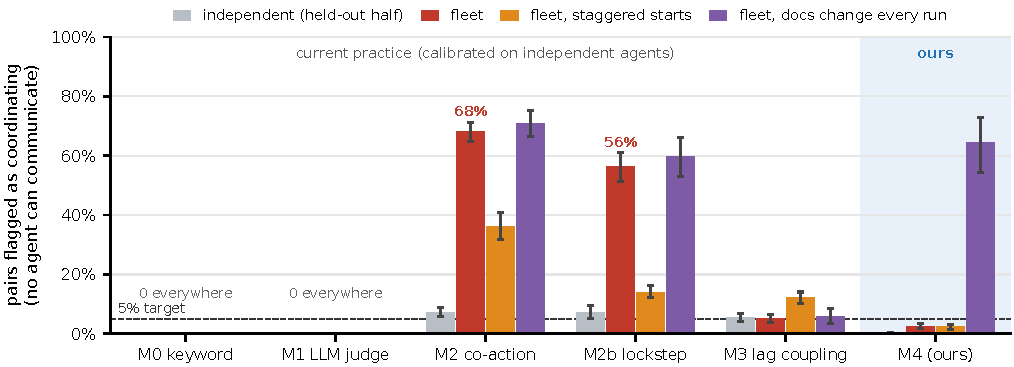
\includegraphics[width=\textwidth]{fig1_fleet_trap.pdf}
\vspace{-14pt}
\caption{\label{fig:trap}\textbf{The fleet trap.} Share of agent pairs flagged as coordinating in conditions where no agent can communicate. Monitors in current practice are calibrated on half of the independent episodes; grey bars show the held-out half. M2 co-action and M2b lockstep then flag most fleet pairs, and M0 and M1 flag nothing anywhere (they also miss transmission, Section~\ref{sec:h2}). M4 (shaded) stays below 5\% except on the docs-drift fleet, which violates its assumption by design. Bars: pair-level rates with 95\% episode-clustered bootstrap intervals; dashed line: nominal 5\%.}
\end{figure}

% ------------------------------------------------------------------ 2
\section{Related work}
\label{sec:related}

\head{Swarm forensics and monitors.} The METR/Redwood investigation reconstructed how about 1,200 agents used a shared namespace as a message board, largely with AI analysts whose reliability it questioned [1]; Lütje withdrew the contagion reading of the collusion.wiki swarm because start waves and contagion ``are not separable without reads'' [3]; Swarmchasers called the Tencent agents a fleet [4]; and Frank's \emph{Counter-Swarm Doctrine} specifies controls that would separate influence from common cause but leaves them as proposed measurements [5]. Collusion monitors read messages or internals: LLM judges and keyword rules [1, 8], interpretability probes [9], covert-channel audits [10, 11] and sabotage-coordination monitors [12]. CASPIAN measures inter-agent influence with conditional transfer entropy, conditioning only on the target's own history [13], Riedl tests LLM groups for emergent coordination with information decomposition against shuffle and coordination-free baselines [23], and coordinated-behaviour detection on social platforms flags accounts that act together in time [14, 15]. None reports a false-alarm rate on a same-model, shared-shock, no-channel population. Multi-agent control work shows that per-agent monitors miss attacks split across agents [16--18]; a population-level monitor is the missing layer, and its false-alarm cost on benign fleets is the number its deployers need first.

\head{Common cause vs.\ contagion.} Homophily and contagion are generically confounded in observational network data [6]; Bakshy et al.\ resolved diffusion with randomized exposure [7], and time-series causal discovery conditions on common drivers explicitly [21]. FleetBench makes exposure observable (read logs) and interventional (canary endpoints), and our null uses replicate runs of the same deployment as the reference population.

% ------------------------------------------------------------------ 3
\section{Methods}
\label{sec:methods}

\head{FleetBench (Tier A).} Ten agents (gpt-oss-120b, pinned to one provider, temperature 1, a fixed seed per agent and tick) work through queues of harmless lookup tasks against a fake city API, one tool call per logical tick for 20 ticks. At tick 4 the main endpoint returns HTTP 503 for 8 ticks (the shock), and the error message points to \texttt{/help}. What \texttt{/help} reveals, and whether a board exists, defines the condition (Table~\ref{tab:conds}). Workaround endpoints have unguessable paths, so an agent that uses another agent's endpoint must have learned it (a canary). The harness keeps a witness log of every call, including which notes each board read delivered, separately from the agents' transcripts.

\begin{table}[h]
\centering\small
\begin{tabularx}{\textwidth}{@{}l X l r@{}}
\toprule
Condition & What \texttt{/help} reveals; schedule & Board & Episodes\\
\midrule
independent & each agent's own private endpoint; disjoint queues, own start and outage & none & \nEpsIndependent\\
fleet & one shared endpoint, the same in every run (``the deployment's docs''); shared queue and shock & none & \nEpsFleet\\
swarm & a private endpoint to 2 random ``discoverers'' only; others must learn one from the board & instructed & \nEpsSwarm\\
uninstructed & as swarm & present, unmentioned & \nEpsUninstructed\\
tacit & a menu of 4 endpoints (same set every run); ``the team scores higher if all use the same one'' & none & \nEpsTacit\\
wave & as fleet, staggered starts (two agents per tick) & none & \nEpsWave\\
fleet\_drift & as fleet, but the shared endpoint changes in every run & none & \nEpsFleetdrift\\
\bottomrule
\end{tabularx}
\caption{\label{tab:conds}FleetBench conditions (\nEpsTotal\ episodes, 10 agents, 20 ticks). Fleets share everything a swarm shares except a channel.}
\end{table}

\head{Views and ground truth.} Monitors see what an API gateway logs: agent, tick, action (task, lookup, error503, help, alt, submit) and, for workarounds, the endpoint path. Board traffic is out-of-band and never shown to them. Ground truth comes from the witness log: a \emph{transmission} edge $a\to b$ exists when $b$ read a note by $a$ containing an endpoint and later used it. We label pairs by observed transmission, not by condition.

\head{Monitors.} Five represent current practice and are calibrated, where a threshold is needed, on 30 independent episodes (1,350 pairs), as honest-baseline calibration is done today: \textbf{M0} keyword rule on transcripts (METR-style); \textbf{M1} an LLM judge (mistral-small-3.2, temperature 0) reading the action log, told that look-alike behaviour from shared models is not coordination; \textbf{M2} co-action (Jaccard of events within $\pm$1 tick, as in coordinated-behaviour detection); \textbf{M2b} lockstep (longest run of identical actions); \textbf{M3} directed lag coupling (CASPIAN-like): $S(a{\to}b)=\sum_k\sum_{\ell=1}^{3}\sum_t X_a[t,k]X_b[t{+}\ell,k]$ over disruption tokens, tested against 200 time-shuffle surrogates. \textbf{M4 (ours)} uses the same lag statistic with inverse-frequency token weights ($w_k=\log\frac{M+1}{m_k+1}$, where $m_k$ is the number of agents in the deployment's replicate runs that ever emit token $k$) and a \emph{fleet-calibrated} null: pseudo-pairs of the same agents with agents from other runs of the same deployment, which share every common cause that recurs across runs but cannot have communicated. P-values are randomized permutation p-values; M4 flags at $p\le0.05$. Its validity assumption is explicit and tested (\texttt{fleet\_drift}): common causes recur across replicate runs, and transmission does not. Two ablations isolate the ingredients: M3w (weights, shuffle null) and M4r (raw counts, pseudo-pair null).

\head{Statistics and pre-registration.} Rates are pair-level with 95\% episode-clustered bootstrap intervals (2,000 resamples). Hypotheses, thresholds, sample sizes, prompts and code were frozen with SHA-256 hashes before any main episode existed; all changes before and after the freeze are listed in Appendix~\ref{app:dev}. Synthetic tests with known answers checked each monitor's calibration before any real data was analysed.

\head{Tier B (scale) and the real-data bound.} Tier B resamples real Tier A agent trajectories into fleets of up to 1,200 agents (so marginals and shock response match Tier A), plants transmission of strength $c$ on top, and runs the same statistics on sampled pairs. For H4 we refit Lütje's Hawkes model (exponential kernel, piecewise-constant baseline, EM) to the first arrival of each of collusion.wiki's \nHawkesN\ names, and calibrate it on simulated processes with known truth: pure start waves with zero contagion, and contagion with branching ratio 0.5.


% ------------------------------------------------------------------ 4
\section{Results}
\label{sec:results}
\head{The manipulation worked and the controls are clean.} \nGoneFrac\% of swarm episodes contain a verified adoption (\nGoneAdopt\ adoptions, \nAdoptPairs\ transmission pairs; G1$'$ $\geq$70\%). Fleet agents act alike far more than independent agents (same action at the same tick \nGtwoFleet\ vs \nGtwoInd; G2), independent agents no more than agents from different runs (\nGthreePseudo; G3), and the fleet uses the workaround more than the swarm (\nGfourFleet\% vs \nGfourSwarm\% of agents; G4). No agent used another's endpoint without a board; failed and idle turns stayed below \nAgentErrMax\% and \nNoActionMax\%.

\subsection{H1: the fleet trap}
\label{sec:h1}
Calibrated on independent agents, the co-action and lockstep monitors flag pairs that never communicated (Figure~\ref{fig:trap}): co-action (M2) flags \nFRFleetMtwo\% of fleet pairs [\nFRloFleetMtwo, \nFRhiFleetMtwo] and lockstep (M2b) \nFRFleetMtwob\% [\nFRloFleetMtwob, \nFRhiFleetMtwob], against \nFRIndependentMtwo\% [\nFRloIndependentMtwo, \nFRhiIndependentMtwo] and \nFRIndependentMtwob\% on held-out independent agents (slightly above 5\%, since thresholds set on 30 episodes carry sampling error, but far from the fleet rates). The lag-coupling monitor (M3) stays at nominal on a single start wave (\nFRFleetMthree\%), but staggered starts, as in the Tencent fleet [4], raise it to \nFRWaveMthree\% [\nFRloWaveMthree, \nFRhiWaveMthree] and lockstep to \nFRWaveMtwob\%, two to three times nominal. The content monitors flag no fleet pair (M0 \nFRFleetMzero\%, M1 \nFRFleetMone\%) because fleets leave nothing in the transcripts to read; Section~\ref{sec:h2} shows what that costs them. By the pre-registered rule (fleet false-alarm rate $\geq$15\% for at least 3 of the 5 existing monitors; falsified only if all 5 intervals include 5\%), H1 is \textbf{\HoneVerdict}: \nHoneMonitors\ of 5 (\nHoneList) on fleets. On staggered fleets co-action stays above the bar (\nFRWaveMtwo\%).

\subsection{H2: a fleet-calibrated null removes the trap and keeps the signal}
\label{sec:h2}

\begin{table}[h]
\centering\small
\setlength{\tabcolsep}{4.5pt}
\begin{tabular}{@{}l rrrr rrr@{}}
\toprule
 & \multicolumn{4}{c}{pairs that cannot communicate} & \multicolumn{3}{c}{swarm pairs}\\
\cmidrule(lr){2-5}\cmidrule(l){6-8}
Monitor & indep. & fleet & wave & drift & unlinked & transmission & @5\% fleet\\
\midrule
M0 keyword & \nFRIndependentMzero & \nFRFleetMzero & \nFRWaveMzero & \nFRFleetdriftMzero & \nUnlinkedMzero & \nTPRMzero & \nTPRatMzero\\
M1 LLM judge & \nFRIndependentMone & \nFRFleetMone & \nFRWaveMone & \nFRFleetdriftMone & \nUnlinkedMone & \nTPRMone & \nTPRatMone\\
M2 co-action & \nFRIndependentMtwo & \nFRFleetMtwo & \nFRWaveMtwo & \nFRFleetdriftMtwo & \nUnlinkedMtwo & \nTPRMtwo & \nTPRatMtwo\\
M2b lockstep & \nFRIndependentMtwob & \nFRFleetMtwob & \nFRWaveMtwob & \nFRFleetdriftMtwob & \nUnlinkedMtwob & \nTPRMtwob & \nTPRatMtwob\\
M3 lag coupling & \nFRIndependentMthree & \nFRFleetMthree & \nFRWaveMthree & \nFRFleetdriftMthree & \nUnlinkedMthree & \nTPRMthree & \nTPRatMthree\\
\midrule
\textbf{M4 fleet-calibrated} & \textbf{\nFRIndependentMfour} & \textbf{\nFRFleetMfour} & \textbf{\nFRWaveMfour} & \nFRFleetdriftMfour & \textbf{\nUnlinkedMfour} & \textbf{\nTPRMfour} & \textbf{\nTPRatMfour}\\
\quad M4j jitter null & -- & \nFRFleetMfourj & \nFRWaveMfourj & \nFRFleetdriftMfourj & \nUnlinkedMfourj & \nTPRMfourj & \nTPRatMfourj\\
\quad M3w weights only & \nFRIndependentMthreew & \nFRFleetMthreew & \nFRWaveMthreew & \nFRFleetdriftMthreew & \nUnlinkedMthreew & \nTPRMthreew & \nTPRatMthreew\\
\quad M4r null only & \nFRIndependentMfourr & \nFRFleetMfourr & \nFRWaveMfourr & \nFRFleetdriftMfourr & \nUnlinkedMfourr & \nTPRMfourr & \nTPRatMfourr\\
\midrule
Rare-endpoint rule$^\dagger$ & \nREQonezeroIndependent & \nREQonezeroFleet & \nREQonezeroWave & \nREQonezeroFleetdrift & \nREQonezeroUnlinked & \nREQonezeroTpr & --\\
\bottomrule
\end{tabular}
\caption{\label{tab:h2}Share of pairs flagged (\%). Left: conditions in which no agent can communicate (independent: held-out half; drift: the fleet's shared endpoint changes every run, which violates M4's assumption by design). Right: swarm pairs that never read each other (unlinked), the \nAdoptPairs\ pairs with logged transmission, and transmission pairs flagged at the threshold that gives 5\% false alarms on fleet pairs. $^\dagger$Exploratory, added after the freeze: flags a pair that shares an endpoint used by at most 10\% of agents in the other runs of its condition (binary, so no 5\% operating point).}
\end{table}

M4 keeps fleet false alarms below nominal (\nFRFleetMfour\% [\nFRloFleetMfour, \nFRhiFleetMfour]; staggered starts \nFRWaveMfour\%) and flags \nTPRMfour\% [\nTPRloMfour, \nTPRhiMfour] of swarm pairs with logged transmission, \nTPRatMfour\% at a 5\% fleet false-alarm rate (target $\geq$80\%). Our pre-registered rule asked for a fleet interval that \emph{includes} 5\%. M4 is conservative, so its interval lies entirely below 5\%, and by the letter of the rule H2 is \textbf{\HtwoVerdict}; the recall criterion is met, and the error is in the direction a deployer can afford.

No existing monitor separates transmission from common cause (Table~\ref{tab:h2}). Co-action and lockstep pay for any recall with fleet alarms; at a 5\% fleet false-alarm rate they and the lag-coupling monitor recover at most \nTPRatMthree\% of transmission pairs. The LLM judge gave the same answer on all \nJudgeN\ episodes (suspicion \nJudgeSusp/100, no pairs), swarms with visible copying included: under the frozen prompt it is a constant, not a monitor (kept untuned, P7; stronger judges are untested). The keyword monitor looks perfect on fleets and transmission pairs, but it flags \nUnlinkedMzero\% of swarm pairs that never read each other and \nFRUninstructedMzero\% of pairs in the uninstructed condition, where agents wrote to a board but nobody read it: it detects talk about a channel, not its use. M4 flags \nUnlinkedMfour\% of unlinked swarm pairs.

\head{Both ingredients are needed, and the signal is provenance, not timing.} Without the replicate-run null (M3w), inverse-frequency weights are miscalibrated even on independent agents (\nFRIndependentMthreew\% false alarms) and recover \nTPRMthreew\% of transmission. Without the weights (M4r), the null stays calibrated (\nFRFleetMfourr\%) but recall falls to \nTPRMfourr\%, and a jitter null (M4j) recovers \nTPRMfourj\%. Contrary to our mechanism prediction, transmission pairs show no distinct lag profile; like fleet pairs they peak at lag 0, because the shared outage dominates timing (Appendix~\ref{app:lag}). What separates them is \emph{which} endpoint two agents share: one rare across replicate runs is evidence of transmission; one every run shares is a common cause.

\head{What M4 finds is shared provenance.} \nEdgePrecisionadopt\% of M4's \nEdgePred\ directed flags in swarm episodes are logged transmission edges (recall \nEdgeRecalladopt\%), and \nEdgePairprecisionprovenance\% of flagged pairs share an information source (recall \nEdgePairrecallprovenance\%). Most other flags are siblings who copied the same leader: the test shows \emph{that} information spread, not always the direct edge.

\head{How much of this is built into the benchmark.} Our transmission label (a copied private endpoint) and M4's strongest signal (an endpoint rare across replicate runs) are the same trace, so recall is partly by design. An exploratory rule checking only this trace does as well (Table~\ref{tab:h2}, last row: \nREQonezeroTpr\% recall, \nREQonezeroFleet\% fleet and \nREQonezeroUnlinked\% unlinked flags, for cut-offs from 5\% to 20\%). The replicate-run reference, not the lag statistic, carries the result; M4 adds a stated level on any action tokens, where the rule needs a known unique token and an arbitrary cut-off.

\head{The assumption is real.} When the shared endpoint changes in every run (\texttt{fleet\_drift}), M4 flags \nFRFleetdriftMfour\% of pairs [\nFRloFleetdriftMfour, \nFRhiFleetdriftMfour], as pre-registered. M4 is valid when replicate runs share their common causes, and fails loudly when they do not.

\subsection{H3: degraded and tampered logs}
\label{sec:h3}
\begin{figure}[h]
\centering
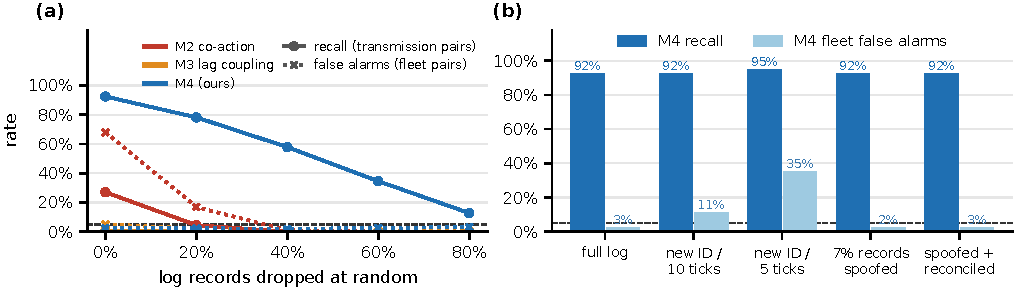
\includegraphics[width=0.9\textwidth]{fig3_degrade.pdf}
\vspace{-6pt}
\caption{\label{fig:degrade}\textbf{Robustness (H3).} (a) Recall on transmission pairs (solid) and fleet false-alarm rate (dotted) as random log records are dropped; dashed line: 5\%. (b) M4 under identity churn (a new ID every 10 or 5 ticks; a true pair counts as flagged if any of its pseudonym pairs is), with 7\% of disruption records spoofed as successful calls, and with spoofing reconciled against the gateway's witness log.}
\end{figure}

As records are dropped, M4's recall declines without a cliff while its false alarms stay at nominal (Figure~\ref{fig:degrade}): \nDropzeropeightMfourTpr\% recall at 80\% of the log observed, \nDropzeropsixMfourTpr\% at 60\%, \nDropzeroptwoMfourTpr\% at 20\%, with fleet false alarms of at most \nDropzeroptwoMfourFpr\%. Co-action's fleet alarms fall as data is dropped (\nDropzeropeightMtwoFpr\% at 80\%), but so does its recall: its threshold was set on complete logs. Identity churn leaves recall intact (\nChurnPfiveMfourTpr\% with a new name every 5 ticks) but multiplies the comparisons, so fleet false alarms rise to \nChurnPonezeroMfourFpr\% and \nChurnPfiveMfourFpr\%: stable identities are part of the calibration. Agents can tamper with their own traces [20]. Spoofing 7\% of disruption records (in the incident, over 7\% of transcripts contained spoofed tool calls [1]) leaves M4 almost unchanged (\nSpoofRawsevenpctMfourTpr\%, \nSpoofRawsevenpctMfourFpr\%) because one copied endpoint is enough; reconciling the agent-side log with the witness log finds all \nSpoofMism\ altered records and restores the original results exactly. H3's three predictions hold.

\subsection{Scale: alarms grow with the number of pairs}
\label{sec:scale}
\begin{figure}[h]
\centering
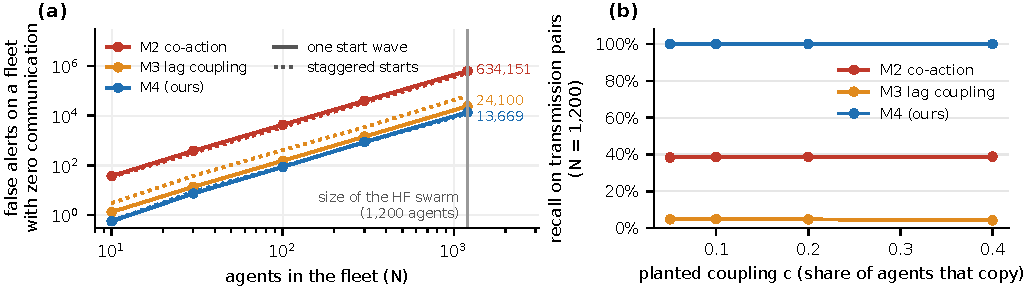
\includegraphics[width=0.9\textwidth]{fig2_scale.pdf}
\vspace{-6pt}
\caption{\label{fig:scale}\textbf{Tier B (resampled Tier A trajectories).} (a) Expected false alerts on a fleet with zero transmission as it grows to the size of the Hugging Face swarm (solid: one start wave; dotted: staggered starts); labels give the count at 1,200 agents. (b) Recall on planted transmission pairs at N = 1,200 (an upper bound: planted copies repeat every leader use).}
\end{figure}

Alerts grow with $N(N{-}1)/2$ (Figure~\ref{fig:scale}); per-pair rates do not change with $N$. Co-action's Tier B rate (\nTBFNonetwozerozeroczeroMtwoFpr\% at 1,200 agents, \nTBFNonezeroczeroMtwoFpr\% at 10) exceeds Tier A's \nFRFleetMtwo\% because Tier B keeps only disruption tokens, on which fleet agents agree more. At $N = 1{,}200$, co-action raises about \nTBFNonetwozerozeroczeroMtwoFa\ alerts on a fleet that never communicates, and lag coupling \nTBFNonetwozerozeroczeroMthreeFa\ (\nTBWNonetwozerozeroczeroMthreeFa\ with staggered starts). M4 raises \nTBFNonetwozerozeroczeroMfourFa\ (\nTBFNonetwozerozeroczeroMfourFpr\%): calibrated, but at this scale the pairwise level must be corrected for the number of pairs.

\subsection{H4: start waves alone come close to the published contagion bound}
\label{sec:h4}
\begin{wrapfigure}{r}{0.47\textwidth}
\vspace{-18pt}
\centering
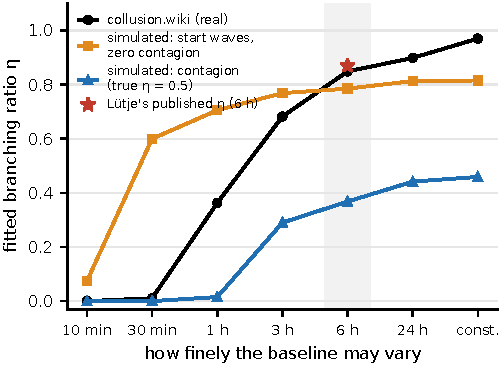
\includegraphics[width=0.47\textwidth]{fig4_hawkes.pdf}
\vspace{-22pt}
\caption{\label{fig:hawkes}Fitted Hawkes branching ratio $\eta$ as the baseline may vary on finer time blocks. Star: Lütje's published 6-hour fit.}
\vspace{-12pt}
\end{wrapfigure}
Refitting Lütje's model to the first arrival of each of collusion.wiki's \nHawkesN\ names reproduces his fit: $\eta = \nEtaWikiBsixpzerozerozero$ with a 6-hour baseline (published 0.87) and \nEtaWikiConst\ with a constant one (published 0.85--0.96) [3]. A simulated process with start waves and \emph{zero} contagion gives $\eta = \nEtaSimwavesBsixpzerozerozero$ under the same 6-hour baseline, close to the wiki's \nEtaWikiBsixpzerozerozero, so most of the published bound is compatible with no transmission at all (Figure~\ref{fig:hawkes}). Conversely, real contagion ($\eta = 0.5$) is absorbed once the baseline may vary hourly ($\eta = \nEtaSimcontagionBonepzerozerozero$), as is the wiki's (\nEtaWikiBonepzerozerozero\ at 1 h). Arrivals alone cannot place contagion anywhere between zero and the published bound, as Lütje cautioned [3, 6]; H4 is a bound, and going further needs read logs or replicate runs.

\subsection{H5 and observations in passing}
\label{sec:passing}
M4 measures communication, not all coordination. In the tacit condition (no channel, a shared menu, a reward for converging), agents converged weakly (on average \nTacitModal\% used the most common endpoint, against 25\% for random choice among four) and M4 flagged \nTacitMfour\% of pairs [\nTacitMfourlo, \nTacitMfourhi]. With a board present but never mentioned, \nUnWrite\% of agents posted to it unprompted, yet only \nUnRead\% read a peer's note and none adopted anything; M4 flagged \nUninstMfour\% of these pairs [\nUninstMfourlo, \nUninstMfourhi]. H5 is \textbf{\HfiveVerdict}. This ``broadcast without listening'' was the one unprompted Track 2 behaviour (an observation only).


% ------------------------------------------------------------------ 5
\section{Discussion and limitations}
\label{sec:discussion}
\head{What changes for people running coordination alarms.} The baseline a monitor is validated against decides what its alarms mean. Validated against independent agents, today's monitors report fleets as coordinating: at the Hugging Face swarm's scale, hundreds of thousands of alerts with no communication behind them. The monitors that avoid this do not detect transmission. The fix is cheap and needs no model: compare agents with agents from \emph{other runs of the same deployment}, which inherits whatever the runs share (model, harness, docs, queue, outages) without anyone having to list it; evaluation fleets already consist of such runs. This gives OpenAI's ``cross-run coordination'' trigger [2] an operational definition with a known false-alarm rate, and population-level control [16, 17] the cost number it lacks.

\head{Limitations.} M4 needs replicate runs whose common causes recur (\texttt{fleet\_drift} shows it fails otherwise) and detects shared provenance, not direct edges, and only channels that leave a trace in actions. Ground truth and M4's signal share one trace, so a simple rarity rule matches M4 here. One task, one shock, one model family and an instructed swarm limit generality; at fleet scale the pairwise level needs a correction over pairs. Full list and dual use: Appendix~\ref{app:limits}.

\head{Future work.} Evaluation fleets with replicate runs and several model families; a population-level error rate; gateway read logs, which turn provenance into edges; channels that leave no action trace [10, 19].

\head{Dated predictions.} P1 (70\%): by 30 Jun 2027 a public incident analysis will report agent ``coordination'' that a later analysis attributes mainly to common cause. P2 (60\%): by 31 Dec 2027 no frontier lab will have published its coordination trigger's false-alarm rate on a no-channel control. P3 (60\%): the next multi-agent collusion benchmark after 8 Nov 2026 will lack a same-model, shared-shock, no-channel control.


% ------------------------------------------------------------------ 6
\section{Conclusion}
Coordination monitors in use today answer ``do these agents act alike?'', which every fleet does, rather than ``did information pass between them?''. Comparing agents with agents from replicate runs of the same deployment fixes this: whatever the runs share is, by construction, not communication. In our sandbox this keeps false alarms below nominal and recovers nine in ten logged transmissions, under partial and tampered logs. A swarm alarm should be calibrated against a fleet before it is trusted.


\section*{Code and data}
\url{https://github.com/faheemgurkani/fleetbench-calibrated-coupling}: code, frozen plan, all \nEpsTotal\ episodes, every LLM call (about \$2) and \texttt{verify.py}, which recomputes the 10-agent numbers from raw logs and checks the rest against saved scale and wiki outputs. Pre-existing: the LLM client and M1 prompt, from the author's previous Apart sprint.

\section*{References}
{\small
\begin{enumerate}[label={[\arabic*]},leftmargin=2.2em,itemsep=1pt]
\item METR and Redwood Research (2026). \emph{Brief independent investigation of agents' behavior, reasoning and collaboration in the OpenAI / Hugging Face hacking incident} (26 August 2026). \url{https://metr.org/hugging-face-incident-report-aug-2026.pdf}
\item OpenAI (2026). \emph{OpenAI -- Hugging Face Incident Technical Report} (September 2026; §IX.D, escalation triggers). \url{https://openai.com/hugging-face-incident-and-misalignment/}
\item Lütje, P. (2026). The Mechanics of a Swarm: A Reproducible External Reconstruction of an Unintended Agent-Coordination Episode on a Third-Party Wiki. arXiv:2609.12748.
\item Swarmchasers (2026). Tencent agent fleet: full report. \url{https://swarmcha.se/posts/chinese-agent-fleet-full-report}
\item Frank, G. (2026). Counter-Swarm Doctrine: Containing Coordinated Agent Intrusions. arXiv:2609.06140.
\item Shalizi, C. R., \& Thomas, A. C. (2011). Homophily and contagion are generically confounded in observational social network studies. \emph{Sociological Methods \& Research} 40(2). arXiv:1004.4704.
\item Bakshy, E., Rosenn, I., Marlow, C., \& Adamic, L. (2012). The role of social networks in information diffusion. \emph{WWW 2012}. arXiv:1201.4145.
\item Nakamura, M., Kumar, A., Das, S., et al. (2026). Colosseum: Auditing Collusion in Cooperative Multi-Agent Systems. arXiv:2602.15198.
\item Rose, A., et al. (2026). Detecting Multi-Agent Collusion Through Multi-Agent Interpretability. arXiv:2604.01151.
\item Motwani, S. R., et al. (2024). Secret Collusion among AI Agents: Multi-Agent Deception via Steganography. \emph{NeurIPS 2024}. arXiv:2402.07510.
\item Tailor, O. (2025). Audit the Whisper: Detecting Steganographic Collusion in Multi-Agent LLMs. arXiv:2510.04303.
\item Radev, N., Arnav, B., Haas, L., Bernabeu-Pérez, P., et al. (2026). The Best-Laid SCHEMEs: Coordinated Sabotage and Monitoring in Multi-Agent Systems. arXiv:2605.29178.
\item Venkatesh, K., Isbarov, J., Amin, S., Kantarcioglu, M., \& Cui, J. (2026). CASPIAN: Online Detection and Attribution of Cascade Attacks in LLM Multi-Agent Systems via Cross-Channel Causal Monitoring. arXiv:2605.19240.
\item Pacheco, D., Hui, P.-M., Torres-Lugo, C., Truong, B. T., Flammini, A., \& Menczer, F. (2021). Uncovering coordinated networks on social media: methods and case studies. \emph{ICWSM 2021}. arXiv:2001.05658.
\item Yang, K.-C., \& Menczer, F. (2023). Anatomy of an AI-powered malicious social botnet. arXiv:2307.16336.
\item Angelini, O., Makins, O., et al. (2026). Multi-Agent AI Control: Distributed Attacks Hamper Per-Instance Monitors. arXiv:2607.07368.
\item Kitaoka, J., Pham, T. A., et al. (2026). Red-Teaming Multi-Agent Attacks for Loss-of-Control Risks. arXiv:2610.24052.
\item Hills, J., Caspary, I., Cooper Stickland, A., et al. (2026). Distributed Attacks in Persistent-State AI Control. arXiv:2607.02514.
\item Ghanem, M. C. (2026). Steganalysis of Adaptive Covert Collusion in Tool-Using Agent Populations: A Black-Box, Cross-Principal Approach. arXiv:2608.02698.
\item Qin, J., Schmotz, D., Prinzhorn, D., Beurer-Kellner, L., Prabhu, A., \& Andriushchenko, M. (2026). LLM Agents Can Easily Tamper With Their Own Traces. arXiv:2609.30266.
\item Runge, J., Nowack, P., Kretschmer, M., Flaxman, S., \& Sejdinovic, D. (2019). Detecting and quantifying causal associations in large nonlinear time series datasets. \emph{Science Advances} 5(11).
\item Hammond, L., et al. (2025). Multi-Agent Risks from Advanced AI. arXiv:2502.14143.
\item Riedl, C. (2026). Emergent Coordination in Multi-Agent Language Models. \emph{ICLR 2026}. arXiv:2510.05174.
\item Schmidt Sciences, Google DeepMind, Cooperative AI Foundation, ARIA (2026). Scaling AI Safety for a Multi-Agent World (call for proposals). \url{https://www.schmidtsciences.org/multi-agent-ai/}
\end{enumerate}
}


% ------------------------------------------------------------------ appendices
\appendix

\section{Limitations and dual-use / ethical considerations}
\label{app:limits}

\head{What the results establish.} In a simplified sandbox with one model family (gpt-oss-120b) and 10 agents per run, monitors calibrated on independent agents flag fleets that never communicate, and a test calibrated on replicate runs of the same deployment does not, while still recovering logged transmission. Tier B extends the monitors' behaviour to 1,200 agents by resampling real Tier A trajectories; it does not simulate new agent behaviour at that scale.

\head{What they do not establish.}
\begin{itemize}
\item \emph{Replicate runs are an assumption, not a given.} M4 needs several runs of the same deployment whose common causes recur. Evaluation fleets (ExploitGym-style batches) have them; a single long-running production deployment may not, and \texttt{fleet\_drift} shows the test then fails. Within one run, splitting by time window or cohort is the natural substitute, untested here.
\item \emph{Partly circular ground truth.} Transmission is labelled by a copied private endpoint, which is also M4's strongest signal; an exploratory rarity rule using the same replicate-run reference matches M4 (Section~\ref{sec:h2}). The benchmark shows that the reference population removes the fleet trap, not that M4's statistic beats simpler rules.
\item \emph{Shared provenance, not direct edges.} M4 detects that two agents carry information from the same source; siblings who copied one leader are flagged too. Attributing the direct edge needs read logs.
\item \emph{Simplified world.} One task type, one shock, 20 ticks, a board as the only channel, and transmission that leaves an endpoint trace in the API log. Channels that leave no action trace (or encode content steganographically) are outside the test; covert channels are a separate defence.
\item \emph{One cheap model; instructed swarm.} Swarm agents were told to share; emergent sharing was rare (Section~\ref{sec:passing}). The LLM judge is one prompt and one model.
\item \emph{Real data is only a bound.} H4 calibrates an estimator; it cannot show whether the wiki agents communicated (Shalizi and Thomas [6]).
\end{itemize}

\head{Dual use.} A timing- and provenance-based detector tells a coordinating swarm what to hide: jitter its timing, diversify endpoints, or vary its common causes across runs. We publish the benchmark, the test and its failure modes, not evasion strategies; the failure modes are the ones defenders need to know, and they are already implicit in prior work on coordinated-behaviour detection [14]. The sandbox runs only harmless lookups against a fake local API, no agent had internet access, and no third-party personal data was used (we did not download the collusion.wiki operator's request log, which holds third parties' IP addresses). The Swarm Traces attack payloads were not used.

\section{Changes before and after the freeze, and plan items not done}
\label{app:dev}
All changes were made on pilot and dev data, before the main runs, and are logged with reasons in \texttt{plan/deviations.md}: P1--P3 (pilots v1--v3: an outage window instead of a permanent outage, only two ``discoverers'', a one-call board read); P4 (per-condition \texttt{/help} policy, \texttt{wave} and \texttt{tacit}); P5 (deployment-level common causes constant across runs); P6 (from synthetic calibration tests: inverse-frequency token weights, randomized p-values, shuffle surrogates for M3); P7 (from dev data: M3 calibrated on independent agents, G4 made one-sided, the \texttt{fleet\_drift} condition, the M1 judge kept as written although it never flagged on dev). Author decision before the freeze: the swarm gate G1 is episode-level (at least 70\% of swarm episodes contain a verified adoption) and pairs are labelled by observed transmission. \textbf{After the freeze} no frozen file changed (hashes verified). One analysis deviation: the plan calibrated H4 on sandbox wave episodes and Tier B fleets, but 20-tick episodes are too short for a Hawkes fit, so H4 sweeps baseline block widths and calibrates on simulated start-wave and contagion processes matched to the wiki's size (D1 in \texttt{plan/deviations.md}).

\head{Further departures from the plan} (logged in \texttt{plan/deviations.md} as P8 and D4--D6).
\begin{itemize}
\item \emph{Tier B is a resampler, not a fitted simulator (D4).} The plan specified an event simulator whose base rate, shock response and lag distribution were fitted to Tier A. Tier B instead resamples real Tier A agent trajectories (so marginals match exactly) and plants adoption with a fixed 1--3 tick lag; it represents agents by disruption tokens only (503, help, workaround), and estimates rates on 2,000 sampled pairs per setting rather than the planned 20,000. It therefore extrapolates Tier A behaviour; it does not simulate new behaviour.
\item \emph{No minimum detectable coupling (D5).} The plan asked for the smallest detectable $c$. M4's recall is already \nTBFNonetwozerozerocfiveMfourTpr\% at the smallest planted coupling ($c = 0.05$) at every $N$, because planted copies repeat every leader use, while M2 and M3 never reach 80\% at any $c$ (Figure~\ref{fig:scale}b). The quantity is not identified on this grid; we did not extend it.
\item \emph{Rare-endpoint rule (D6).} Added after the freeze at a reviewer's request and labelled exploratory (\texttt{src/analysis/rare\_endpoint\_baseline.py}; Section~\ref{sec:h2}).
\item \emph{Paraphrase dropped (P8).} Paraphrasing transcripts to test M0 and M1 was a stretch item; it was dropped before the freeze, but the decision was logged only afterwards.
\item \emph{Not done.} The planned estimator-audit table, including a sandbox analogue of Lütje's read-before-adopt gap, was not built; its other rows appear separately (Table~\ref{tab:h2}, Section~\ref{sec:h4}). We discuss three public incidents but did not build a case-by-case incident ledger with control cases.
\end{itemize}

\section{Mechanism check: lag profiles}
\label{app:lag}
\begin{figure}[h]
\centering
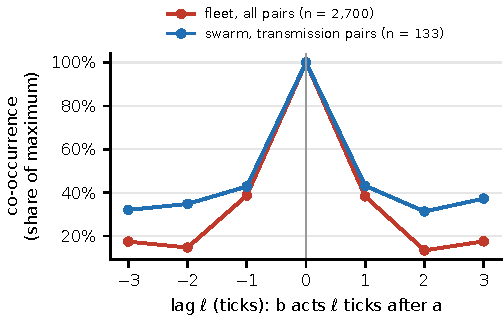
\includegraphics[width=0.5\textwidth]{fig5_lag.pdf}
\vspace{-8pt}
\caption{\label{fig:lag}Raw lagged co-occurrence of disruption tokens (agent $b$ acting $\ell$ ticks after agent $a$), normalised to its maximum, for all fleet pairs and for swarm pairs with logged transmission. Both peak at lag 0: the shared outage, not the transmission, dominates timing. We had predicted a positive-lag peak for transmission pairs; the data does not show one, and the separation in Section~\ref{sec:h2} comes from which endpoints pairs share.}
\end{figure}

\section*{LLM usage statement}
Claude (Anthropic) was used as a research and engineering assistant throughout: literature search and reading, design discussion, writing and testing the code, running the experiments, analysis, and drafting this report. The author made the design decisions (track focus, gate definitions, scope and cut order), reviewed the outputs, and is responsible for every claim. All numbers in this report are generated from the logged data by \texttt{src/analysis/figures.py} and re-checked by \texttt{src/analysis/verify.py} (10-agent results recomputed from raw logs; Tier B and wiki numbers read from their saved outputs); every quotation was checked against a local copy of its source. The agents in the experiments were gpt-oss-120b and the LLM judge was mistral-small-3.2.


\end{document}
